% !TeX spellcheck = de_DE
\documentclass[a4paper,14pt]{extreport}

%%% Проверка используемого TeX-движка %%%
\usepackage{iftex}
\newif\ifxetexorluatex   % определяем новый условный оператор (http://tex.stackexchange.com/a/47579/79756)
\ifXeTeX
    \xetexorluatextrue
\else
    \ifLuaTeX
        \xetexorluatextrue
    \else
        \xetexorluatexfalse
    \fi
\fi

%%% Поля и разметка страницы %%%
\usepackage{pdflscape}                              % Для включения альбомных страниц
\usepackage{geometry}                               % Для последующего задания полей

%%% Математические пакеты %%%
\usepackage{amsthm,amsfonts,amsmath,amssymb,amscd}  % Математические дополнения от AMS
\usepackage{mathtools}                              % Добавляет окружение multlined

%%%% Установки для размера шрифта 14 pt %%%%
%% Формирование переменных и констант для сравнения (один раз для всех подключаемых файлов)%%
%% должно располагаться до вызова пакета fontspec или polyglossia, потому что они сбивают его работу
\newlength{\curtextsize}
\newlength{\bigtextsize}
\setlength{\bigtextsize}{13.9pt}

\makeatletter
%\show\f@size                                       % неплохо для отслеживания, но вызывает стопорение процесса, если документ компилируется без команды  -interaction=nonstopmode 
\setlength{\curtextsize}{\f@size pt}
\makeatother

%%% Кодировки и шрифты %%%
\ifxetexorluatex
    \usepackage{polyglossia}                        % Поддержка многоязычности (fontspec подгружается автоматически)
\else
    \RequirePDFTeX                                  % tests for PDFTEX use and throws an error if a different engine is being used
   %%% Решение проблемы копирования текста в буфер кракозябрами
%    \input glyphtounicode.tex
%    \input glyphtounicode-cmr.tex %from pdfx package
%    \pdfgentounicode=1
    \usepackage{cmap}                               % Улучшенный поиск русских слов в полученном pdf-файле
    \defaulthyphenchar=127                          % Если стоит до fontenc, то переносы не впишутся в выделяемый текст при копировании его в буфер обмена
    \usepackage[T2A]{fontenc}                       % Поддержка русских букв
    \usepackage[utf8]{inputenc}                     % Кодировка utf8
    \usepackage[english, russian]{babel}            % Языки: русский, английский
    \IfFileExists{pscyr.sty}{\usepackage{pscyr}}{}  % Красивые русские шрифты
\fi

%%% Оформление абзацев %%%
\usepackage{indentfirst}                            % Красная строка

%%% Цвета %%%
\usepackage[dvipsnames,usenames]{color}
\usepackage{colortbl}
%\usepackage[dvipsnames, table, hyperref, cmyk]{xcolor} % Вероятно, более новый вариант, вместо предыдущих двух строк. Конвертация всех цветов в cmyk заложена как удовлетворение возможного требования типографий. Возможно конвертирование и в rgb.
\usepackage{soul}

%%% Таблицы %%%
\usepackage{longtable}                              % Длинные таблицы
\usepackage{multirow,makecell,array}                % Улучшенное форматирование таблиц
\usepackage{booktabs}                               % Возможность оформления таблиц в классическом книжном стиле (при правильном использовании не противоречит ГОСТ)

%%% Общее форматирование
\usepackage{soulutf8}                               % Поддержка переносоустойчивых подчёркиваний и зачёркиваний
\usepackage{icomma}                                 % Запятая в десятичных дробях


%%% Гиперссылки %%%
\usepackage{hyperref}

%%% Изображения %%%
\usepackage{graphicx}                               % Подключаем пакет работы с графикой

%%% Списки %%%
\usepackage{enumitem}

%%% Подписи %%%
\usepackage{caption}                                % Для управления подписями (рисунков и таблиц) % Может управлять номерами рисунков и таблиц с caption %Иногда может управлять заголовками в списках рисунков и таблиц
\usepackage{subcaption}                             % Работа с подрисунками и подобным

%%% Интервалы %%%
\usepackage[onehalfspacing]{setspace}               % Опция запуска пакета правит не только интервалы в обычном тексте, но и формульные

%%% Счётчики %%%
\usepackage[figure,table]{totalcount}               % Счётчик рисунков и таблиц
\usepackage{totcount}                               % Пакет создания счётчиков на основе последнего номера подсчитываемого элемента (может требовать дважды компилировать документ)
\usepackage{totpages}                               % Счётчик страниц, совместимый с hyperref (ссылается на номер последней страницы). Желательно ставить последним пакетом в преамбуле

%%% Продвинутое управление групповыми ссылками (пока только формулами) %%%
\ifxetexorluatex
    \usepackage{cleveref}                           % cleveref корректно считывает язык из настроек polyglossia
\else
    \usepackage[russian]{cleveref}                  % cleveref имеет сложности со считыванием языка из babel. Такое решение русификации вывода выбрано вместо определения в documentclass из опасности что-то лишнее передать во все остальные пакеты, включая библиографию.
\fi
\creflabelformat{equation}{#2#1#3}                  % Формат по умолчанию ставил круглые скобки вокруг каждого номера ссылки, теперь просто номера ссылок без какого-либо дополнительного оформления

%%% Колонтитулы %%%
\usepackage{fancyhdr}

%%% Прикладные пакеты %%% 
\usepackage{calc}               % Пакет для расчётов параметров, например длины
%\usepackage{etoolbox}          % ради функции patchcmd для управления списком литературы

\usepackage {interfaces-base}   % Набор базовых интерфейсов к некоторым пакетам, конкретные реализации загружаются в стиле

%%% Заголовки %%%
\usepackage{titlesec}           % Пакет настройки шрифтов заголовков в тексте

%%% Оглавление %%%
\usepackage{tocloft}

%%% Счётчики %%%
\usepackage{chngcntr}           % оперативная перенастройка счётчиков

\usepackage{tabularx,tabulary}  %таблицы с автоматически подбирающейся шириной столбцов

% Листинги с исходным кодом программ
\usepackage{fancyvrb}
\usepackage{listings}

% Плавающие окружения. во многом лучше пакета float
\usepackage{floatrow}

% Русская традиция начертания греческих букв
%\usepackage{upgreek} % прямые греческие ради русской традиции

\usepackage{siunitx}
\sisetup{
	locale=UK,
	%   mode=text,% when using a font without math support
}
  
%%%%%%%%%%%%%%%%%%%%%%%%%%%%%%%%%%%%%%%%%%%%%%%%%%%%%%
%%%% Файл упрощённых настроек шаблона диссертации %%%%
%%%%%%%%%%%%%%%%%%%%%%%%%%%%%%%%%%%%%%%%%%%%%%%%%%%%%%

%%%        Подключение пакетов                 %%%
\usepackage{ifthen}                 % добавляет ifthenelse
%%% Инициализирование переменных, не трогать!  %%%
\newcounter{intvl}
\newcounter{otstup}
\newcounter{contnumeq}
\newcounter{contnumfig}
\newcounter{contnumtab}
\newcounter{pgnum}
\newcounter{bibliosel}
\newcounter{chapstyle}
\newcounter{headingdelim}
\newcounter{headingalign}
\newcounter{headingsize}
\newcounter{tabcap}
\newcounter{tablaba}
\newcounter{tabtita}
%%%%%%%%%%%%%%%%%%%%%%%%%%%%%%%%%%%%%%%%%%%%%%%%%%

%%% Область упрощённого управления оформлением %%%

%% Интервал между заголовками и между заголовком и текстом
% Заголовки отделяют от текста сверху и снизу тремя интервалами (ГОСТ Р 7.0.11-2011, 5.3.5)
\setcounter{intvl}{3}               % Коэффициент кратности к размеру шрифта

%% Отступы у заголовков в тексте
\setcounter{otstup}{0}              % 0 --- без отступа; 1 --- абзацный отступ

%% Нумерация формул, таблиц и рисунков
\setcounter{contnumeq}{0}           % Нумерация формул: 0 --- пораздельно (во введении подряд, без номера раздела); 1 --- сквозная нумерация по всей диссертации
\setcounter{contnumfig}{0}          % Нумерация рисунков: 0 --- пораздельно (во введении подряд, без номера раздела); 1 --- сквозная нумерация по всей диссертации
\setcounter{contnumtab}{1}          % Нумерация таблиц: 0 --- пораздельно (во введении подряд, без номера раздела); 1 --- сквозная нумерация по всей диссертации

%% Оглавление
\setcounter{pgnum}{1}               % 0 --- номера страниц никак не обозначены; 1 --- Стр. над номерами страниц (дважды компилировать после изменения)

%% Библиография
\setcounter{bibliosel}{1}           % 0 --- встроенная реализация с загрузкой файла через движок bibtex8; 1 --- реализация пакетом biblatex через движок biber

%% Текст и форматирование заголовков
\setcounter{chapstyle}{1}           % 0 --- разделы только под номером; 1 --- разделы с названием "Глава" перед номером
\setcounter{headingdelim}{1}        % 0 --- номер отделен пропуском в 1em или \quad; 1 --- номера разделов и приложений отделены точкой с пробелом, подразделы пропуском без точки; 2 --- номера разделов, подразделов и приложений отделены точкой с пробелом.

%% Выравнивание заголовков в тексте
\setcounter{headingalign}{0}        % 0 --- по центру; 1 --- по левому краю

%% Размеры заголовков в тексте
\setcounter{headingsize}{0}         % 0 --- по ГОСТ, все всегда 14 пт; 1 --- пропорционально изменяющийся размер в зависимости от базового шрифта

%% Подпись таблиц
\setcounter{tabcap}{0}              % 0 --- по ГОСТ, номер таблицы и название разделены тире, выровнены по левому краю, при необходимости на нескольких строках; 1 --- подпись таблицы не по ГОСТ, на двух и более строках, дальнейшие настройки: 
%Выравнивание первой строки, с подписью и номером
\setcounter{tablaba}{2}             % 0 --- по левому краю; 1 --- по центру; 2 --- по правому краю
%Выравнивание строк с самим названием таблицы
\setcounter{tabtita}{1}             % 0 --- по левому краю; 1 --- по центру; 2 --- по правому краю

%%% Цвета гиперссылок %%%
% Latex color definitions: http://latexcolor.com/
\definecolor{linkcolor}{rgb}{0,0,1}
\definecolor{citecolor}{rgb}{0,0,1}
\definecolor{urlcolor}{rgb}{0,0,1}
%\definecolor{linkcolor}{rgb}{0.9,0,0}
%\definecolor{citecolor}{rgb}{0,0.6,0}
%\definecolor{urlcolor}{rgb}{0,0,1}
%\definecolor{linkcolor}{rgb}{0,0,0} %black
%\definecolor{citecolor}{rgb}{0,0,0} %black
%\definecolor{urlcolor}{rgb}{0,0,0} %black

% Новые переменные, которые могут использоваться во всём проекте
\newcommand{\authorbibtitle}{Публикации автора по теме диссертации}
\newcommand{\fullbibtitle}{Список литературы} % (ГОСТ Р 7.0.11-2011, 4) 
%%% Основные сведения %%%
\newcommand{\thesisAuthor}             % Диссертация, ФИО автора
{%
    \texorpdfstring{% \texorpdfstring takes two arguments and uses the first for (La)TeX and the second for pdf
        Сидоров Федор Алексеевич% так будет отображаться на титульном листе или в тексте, где будет использоваться переменная
    }{%
        Сидоров, Федор Алексеевич% эта запись для свойств pdf-файла. В таком виде, если pdf будет обработан программами для сбора библиографических сведений, будет правильно представлена фамилия.
    }%
}
\newcommand{\thesisUdk}                % Диссертация, УДК
{\todo{xxx.xxx}}
\newcommand{\thesisTitle}              % Диссертация, название
{\texorpdfstring{\MakeUppercase{Физические механизмы сухого электронно-лучевого травления}}{Физические механизмы сухого электронно-лучевого травления}}
\newcommand{\thesisSpecialtyNumber}    % Диссертация, специальность, номер
{2.2.2}
\newcommand{\thesisSpecialtyTitle}     % Диссертация, специальность, название
{Электронная компонентная база микро- и наноэлектроники, квантовых устройств}
\newcommand{\thesisDegree}             % Диссертация, научная степень
{кандидата физико-математических наук}
\newcommand{\thesisCity}               % Диссертация, город защиты
{Москва}
\newcommand{\thesisYear}               % Диссертация, год защиты
{2023}
\newcommand{\thesisOrganization}       % Диссертация, организация
{Федеральное государственное бюджетное учреждение науки «Физико-технологический институт им. К.А. Валиева Российской академии наук»}

\newcommand{\thesisInOrganization}       % Диссертация, организация в предложном падеже: Работа выполнена в ...
{Федеральном государственном бюджетном учреждении науки «Физико-технологический институт им. К.А. Валиева Российской академии наук»}

\newcommand{\supervisorFio}            % Научный руководитель, ФИО
{Рогожин Александр Евгеньевич}
\newcommand{\supervisorRegalia}        % Научный руководитель, регалии
{кандидат физико-математических наук}

\newcommand{\opponentOneFio}           % Оппонент 1, ФИО
{Чесноков Сергей Артурович}
\newcommand{\opponentOneRegalia}       % Оппонент 1, регалии
{доктор химических наук}
\newcommand{\opponentOneJobPlace}      % Оппонент 1, место работы
{Института металлоорганической химии им. Г.А. Разуваева РАН}
\newcommand{\opponentOneJobPost}       % Оппонент 1, должность
{ведущий научный сотрудник, заведующий Лабораторией фотополимеризации и полимерных материалов}

\newcommand{\opponentTwoFio}           % Оппонент 2, ФИО
{\todo{XXX}}
\newcommand{\opponentTwoRegalia}       % Оппонент 2, регалии
{\todo{регалии}}
\newcommand{\opponentTwoJobPlace}      % Оппонент 2, место работы
{\todo{место работы}}
\newcommand{\opponentTwoJobPost}       % Оппонент 2, должность
{\todo{должность}}

\newcommand{\leadingOrganizationTitle} % Ведущая организация, дополнительные строки
{Государственный научный центр Научно-производственный комплекс ``Технологический центр''}

\newcommand{\defenseDate}              % Защита, дата
{\underline{\hspace{2em}}.\underline{\hspace{2em}}.2023 в \underline{\hspace{2em}}:\underline{\hspace{2em}}}
\newcommand{\defenseCouncilNumber}     % Защита, номер диссертационного совета
{\underline{\hspace{12em}}}
\newcommand{\defenseCouncilTitle}      % Защита, учреждение диссертационного совета
{...}
\newcommand{\defenseCouncilAddress}    % Защита, адрес учреждение диссертационного совета
{...}

\newcommand{\defenseSecretaryFio}      % Секретарь диссертационного совета, ФИО
{}
\newcommand{\defenseSecretaryRegalia}  % Секретарь диссертационного совета, регалии
{регалии}            % Для сокращений есть ГОСТы, например: ГОСТ Р 7.0.12-2011 + http://base.garant.ru/179724/#block_30000

%\textnohyphenation{ФТИАН} им. К.А. Валиева РАН и на сайте института: https://mipt.ru/education/post-graduate/soiskateli-fiziko-matematicheskie-nauki.php

\newcommand{\synopsisLibrary}          % Автореферат, название библиотеки
{	
	\textnohyphenation{ФТИАН} им. К.А. Валиева РАН \kern-0.2em
}
\newcommand{\synopsisDate}             % Автореферат, дата рассылки
{<<\underline{\hspace{2em}}>> \underline{\hspace{8em}} 2023 года}

\newcommand{\keywords}%                 % Ключевые слова для метаданных PDF диссертации и автореферата
{}
%%% Макет страницы %%%
% Выставляем значения полей (ГОСТ 7.0.11-2011, 5.3.7)
\geometry{a4paper,top=2cm,bottom=2cm,left=2.5cm,right=1cm}

%%% Кодировки и шрифты %%%
\ifxetexorluatex
    \setmainlanguage[babelshorthands=true]{russian}  % Язык по-умолчанию русский с поддержкой приятных команд пакета babel
    \setotherlanguage{english}                       % Дополнительный язык = английский (в американской вариации по-умолчанию)
    \ifXeTeX
        \defaultfontfeatures{Ligatures=TeX,Mapping=tex-text}
    \else
        \defaultfontfeatures{Ligatures=TeX}
    \fi
    \setmainfont{Times New Roman}
    \newfontfamily\cyrillicfont{Times New Roman}
    \setsansfont{Arial}
    \newfontfamily\cyrillicfontsf{Arial}
    \setmonofont{Courier New}
    \newfontfamily\cyrillicfonttt{Courier New}
\else
	\IfFileExists{pscyr.sty}{\renewcommand{\rmdefault}{ftm}}{}
%    \IfFileExists{pscyr.sty}{\renewcommand{\rmdefault}{faq}}{}
\fi

%%% Интервалы %%%
%linespread-реализация ближе к реализации полуторного интервала в ворде.
%setspace реализация заточена под шрифты 10, 11, 12pt, под остальные кегли хуже, но всё же ближе к типографской классике. 
%\linespread{1.3}                    % Полуторный интервал (ГОСТ Р 7.0.11-2011, 5.3.6)

%%% Выравнивание и переносы %%%
\sloppy                             % Избавляемся от переполнений
\clubpenalty=10000                  % Запрещаем разрыв страницы после первой строки абзаца
\widowpenalty=10000                 % Запрещаем разрыв страницы после последней строки абзаца

%%% Подписи %%%
\captionsetup{%
singlelinecheck=off,                % Многострочные подписи, например у таблиц
skip=2pt,                           % Вертикальная отбивка между подписью и содержимым рисунка или таблицы определяется ключом
justification=centering,            % Центрирование подписей, заданных командой \caption
}

%%% Рисунки %%%
\DeclareCaptionLabelSeparator*{emdash}{~--- }             % (ГОСТ 2.105, 4.3.1)
\captionsetup[figure]{labelsep=emdash,font=onehalfspacing,position=bottom}

%%% Таблицы %%%
\ifthenelse{\equal{\thetabcap}{0}}{%
    \newcommand{\tabcapalign}{\raggedright}  % по левому краю страницы или аналога parbox
}

\ifthenelse{\equal{\thetablaba}{0} \AND \equal{\thetabcap}{1}}{%
    \newcommand{\tabcapalign}{\raggedright}  % по левому краю страницы или аналога parbox
}

\ifthenelse{\equal{\thetablaba}{1} \AND \equal{\thetabcap}{1}}{%
    \newcommand{\tabcapalign}{\centering}    % по центру страницы или аналога parbox
}

\ifthenelse{\equal{\thetablaba}{2} \AND \equal{\thetabcap}{1}}{%
    \newcommand{\tabcapalign}{\raggedleft}   % по правому краю страницы или аналога parbox
}

\ifthenelse{\equal{\thetabtita}{0} \AND \equal{\thetabcap}{1}}{%
    \newcommand{\tabtitalign}{\raggedright}  % по левому краю страницы или аналога parbox
}

\ifthenelse{\equal{\thetabtita}{1} \AND \equal{\thetabcap}{1}}{%
    \newcommand{\tabtitalign}{\centering}    % по центру страницы или аналога parbox
}

\ifthenelse{\equal{\thetabtita}{2} \AND \equal{\thetabcap}{1}}{%
    \newcommand{\tabtitalign}{\raggedleft}   % по правому краю страницы или аналога parbox
}

\DeclareCaptionFormat{tablenocaption}{\tabcapalign #1\strut}        % Наименование таблицы отсутствует
\ifthenelse{\equal{\thetabcap}{0}}{%
    \DeclareCaptionFormat{tablecaption}{\tabcapalign #1#2#3}
    \captionsetup[table]{labelsep=emdash}                       % тире как разделитель идентификатора с номером от наименования
}{%
    \DeclareCaptionFormat{tablecaption}{\tabcapalign #1#2\par%  % Идентификатор таблицы на отдельной строке
        \tabtitalign{#3}}                                       % Наименование таблицы строкой ниже
    \captionsetup[table]{labelsep=space}                        % пробельный разделитель идентификатора с номером от наименования
}
\captionsetup[table]{format=tablecaption,singlelinecheck=off,font=onehalfspacing,position=top,skip=0pt}  % многострочные наименования и прочее
\DeclareCaptionLabelFormat{continued}{Продолжение таблицы~#2}

%%% Подписи подрисунков %%%
\renewcommand{\thesubfigure}{\asbuk{subfigure}}           % Буквенные номера подрисунков
\captionsetup[subfigure]{font={normalsize},               % Шрифт подписи названий подрисунков (не отличается от основного)
    labelformat=brace,                                    % Формат обозначения подрисунка
    justification=centering,                              % Выключка подписей (форматирование), один из вариантов            
}
%\DeclareCaptionFont{font12pt}{\fontsize{12pt}{13pt}\selectfont} % объявляем шрифт 12pt для использования в подписях, тут же надо интерлиньяж объявлять, если не наследуется
%\captionsetup[subfigure]{font={font12pt}}                 % Шрифт подписи названий подрисунков (всегда 12pt)

%%% Настройки гиперссылок %%%
\ifLuaTeX
    \hypersetup{
        unicode,                % Unicode encoded PDF strings
    }
\fi

\hypersetup{
    linktocpage=true,           % ссылки с номера страницы в оглавлении, списке таблиц и списке рисунков
%    linktoc=all,                % both the section and page part are links
%    pdfpagelabels=false,        % set PDF page labels (true|false)
    plainpages=false,           % Forces page anchors to be named by the Arabic form  of the page number, rather than the formatted form
    colorlinks,                 % ссылки отображаются раскрашенным текстом, а не раскрашенным прямоугольником, вокруг текста
    linkcolor={linkcolor},      % цвет ссылок типа ref, eqref и подобных
    citecolor={citecolor},      % цвет ссылок-цитат
    urlcolor={urlcolor},        % цвет гиперссылок
%    hidelinks,                  % Hide links (removing color and border)
    pdftitle={\thesisTitle},    % Заголовок
    pdfauthor={\thesisAuthor},  % Автор
    pdfsubject={\thesisSpecialtyNumber\ \thesisSpecialtyTitle},      % Тема
%    pdfcreator={Создатель},     % Создатель, Приложение
%    pdfproducer={Производитель},% Производитель, Производитель PDF
    pdfkeywords={\keywords},    % Ключевые слова
    pdflang={ru},
}

%%% Шаблон %%%
\DeclareRobustCommand{\todo}{\textcolor{red}}       % решаем проблему превращения названия цвета в результате \MakeUppercase, http://tex.stackexchange.com/a/187930/79756 , \DeclareRobustCommand protects \todo from expanding inside \MakeUppercase
\setlength{\parindent}{2.5em}                       % Абзацный отступ. Должен быть одинаковым по всему тексту и равен пяти знакам (ГОСТ Р 7.0.11-2011, 5.3.7).

%%% Списки %%%
% Используем дефис для ненумерованных списков (ГОСТ 2.105-95, 4.1.7)
\renewcommand{\labelitemi}{\normalfont\bfseries{--}} 
\setlist{nosep,%                                    % Единый стиль для всех списков (пакет enumitem), без дополнительных интервалов.
    labelindent=\parindent,leftmargin=*%            % Каждый пункт, подпункт и перечисление записывают с абзацного отступа (ГОСТ 2.105-95, 4.1.8)
}

%%% Изображения %%%
\graphicspath{{images/}}         % Пути к изображениям

\LoadInterface {titlesec}                   % Подгружаем интерфейсы для дополнительных опций управления некоторыми пакетами

%%% Блок управления параметрами для выравнивания заголовков в тексте %%%
\newlength{\otstuplen}
\setlength{\otstuplen}{\theotstup\parindent}
\ifthenelse{\equal{\theheadingalign}{0}}{% выравнивание заголовков в тексте
    \newcommand{\hdngalign}{\filcenter}                % по центру
    \newcommand{\hdngaligni}{\hfill\hspace{\otstuplen}}% по центру
}{%
    \newcommand{\hdngalign}{\filright}                 % по левому краю
    \newcommand{\hdngaligni}{\hspace{\otstuplen}}      % по левому краю
} % В обоих случаях вроде бы без переноса, как и надо (ГОСТ Р 7.0.11-2011, 5.3.5)

%%% Оглавление %%%
\renewcommand{\cftchapdotsep}{\cftdotsep}                % отбивка точками до номера страницы начала главы/раздела
\renewcommand{\cfttoctitlefont}{\hdngaligni\fontsize{14pt}{16pt}\selectfont\bfseries}% вместе со следующей строкой
\renewcommand{\cftaftertoctitle}{\hfill}                 % устанавливает заголовок по центру
\setlength{\cftbeforetoctitleskip}{-1.4\curtextsize}     % Поскольку этот заголовок всегда является первым на странице, то перед ним отделять пустым тройным интервалом не следует. Независимо от основного шрифта, в этом случае зануление (почти) происходит при -1.4\curtextsize.
\setlength{\cftaftertoctitleskip}{\theintvl\curtextsize} % Если считаем Оглавление заголовком, то выставляем после него тройной интервал через наше определённое значение

%% Переносить слова в заголовке не допускается (ГОСТ Р 7.0.11-2011, 5.3.5). Заголовки в оглавлении должны точно повторять заголовки в тексте (ГОСТ Р 7.0.11-2011, 5.2.3). Прямого указания на запрет переносов в оглавлении нет, но по той же логике невнесения искажений в смысл, лучше в оглавлении не переносить:
\cftsetrmarg{2.55em plus1fil}                       %To have the (sectional) titles in the ToC, etc., typeset ragged right with no hyphenation
\renewcommand{\cftchappagefont}{\normalfont}        % нежирные номера страниц у глав в оглавлении
\renewcommand{\cftchapleader}{\cftdotfill{\cftchapdotsep}}% нежирные точки до номеров страниц у глав в оглавлении
%\renewcommand{\cftchapfont}{}                       % нежирные названия глав в оглавлении

\ifthenelse{\theheadingdelim > 0}{%
    \renewcommand\cftchapaftersnum{.\ }   % добавляет точку с пробелом после номера раздела в оглавлении
}{%
\renewcommand\cftchapaftersnum{\quad}     % добавляет \quad после номера раздела в оглавлении
}
\ifthenelse{\theheadingdelim > 1}{%
    \renewcommand\cftsecaftersnum{.\ }    % добавляет точку с пробелом после номера подраздела в оглавлении
    \renewcommand\cftsubsecaftersnum{.\ } % добавляет точку с пробелом после номера подподраздела в оглавлении
}{%
\renewcommand\cftsecaftersnum{\quad}      % добавляет \quad после номера подраздела в оглавлении
\renewcommand\cftsubsecaftersnum{\quad}   % добавляет \quad после номера подподраздела в оглавлении
}

\ifthenelse{\equal{\thepgnum}{1}}{%
    \addtocontents{toc}{~\hfill{Стр.}\par}% добавить Стр. над номерами страниц
}

%%% Оформление названий глав %%%
%% настройки заголовка списка рисунков
\renewcommand{\cftloftitlefont}{\hdngaligni\fontsize{14pt}{16pt}\selectfont\bfseries}% вместе со следующей строкой
\renewcommand{\cftafterloftitle}{\hfill}                                             % устанавливает заголовок по центру
\setlength{\cftbeforeloftitleskip}{-1.5\curtextsize}     % Поскольку этот заголовок всегда является первым на странице, то перед ним отделять пустым тройным интервалом не следует. Независимо от основного шрифта, в этом случае зануление (почти) происходит при -1.5\curtextsize.
\setlength{\cftafterloftitleskip}{\theintvl\curtextsize} % выставляем после него тройной интервал через наше определённое значение

%% настройки заголовка списка таблиц
\renewcommand{\cftlottitlefont}{\hdngaligni\fontsize{14pt}{16pt}\selectfont\bfseries}% вместе со следующей строкой
\renewcommand{\cftafterlottitle}{\hfill}                                             % устанавливает заголовок по центру
\setlength{\cftbeforelottitleskip}{-1.5\curtextsize}     % Поскольку этот заголовок всегда является первым на странице, то перед ним отделять пустым тройным интервалом не следует. Независимо от основного шрифта, в этом случае зануление (почти) происходит при -1.5\curtextsize.
\setlength{\cftafterlottitleskip}{\theintvl\curtextsize} % выставляем после него тройной интервал через наше определённое значение

\ifnum\curtextsize>\bigtextsize     % Проверяем условие использования базового шрифта 14 pt
\setlength{\headheight}{17pt}       % Исправляем высоту заголовка
\else
\setlength{\headheight}{15pt}       % Исправляем высоту заголовка
\fi

%%% Колонтитулы %%%
% Порядковый номер страницы печатают на середине верхнего поля страницы (ГОСТ Р 7.0.11-2011, 5.3.8)
\makeatletter
\let\ps@plain\ps@fancy              % Подчиняем первые страницы каждой главы общим правилам
\makeatother
\pagestyle{fancy}                   % Меняем стиль оформления страниц
\fancyhf{}                          % Очищаем текущие значения
\fancyhead[C]{\thepage}             % Печатаем номер страницы на середине верхнего поля
\renewcommand{\headrulewidth}{0pt}  % Убираем разделительную линию

%%% Оформление заголовков глав, разделов, подразделов %%%
%% Работа должна быть выполнена ... размером шрифта 12-14 пунктов (ГОСТ Р 7.0.11-2011, 5.3.8). То есть не должно быть надписей шрифтом более 14. Так и поставим.
%% Эти установки будут давать одинаковый результат независимо от выбора базовым шрифтом 12 пт или 14 пт
\titleformat{\chapter}[block]                                % default display;  hang = with a hanging label. (Like the standard \section.); block = typesets the whole title in a block (a paragraph) without additional formatting. Useful in centered titles
        {\hdngalign\fontsize{14pt}{16pt}\selectfont\bfseries}% 
        %\fontsize{<size>}{<skip>} % второе число ставим 1.2*первое, чтобы адекватно отрабатывали команды по расчету полуторного интервала (домножая разные комбинации коэффициентов на этот)
        {\thechapter\cftchapaftersnum}                       % Заголовки в оглавлении должны точно повторять заголовки в тексте (ГОСТ Р 7.0.11-2011, 5.2.3).
        {0em}% отступ от номера до текста
        {}%

\titleformat{\section}[block]                                % default hang;  hang = with a hanging label. (Like the standard \section.); block = typesets the whole title in a block (a paragraph) without additional formatting. Useful in centered titles
        {\hdngalign\fontsize{14pt}{16pt}\selectfont\bfseries}% 
        %\fontsize{<size>}{<skip>} % второе число ставим 1.2*первое, чтобы адекватно отрабатывали команды по расчету полуторного интервала (домножая разные комбинации коэффициентов на этот)
        {\thesection\cftsecaftersnum}                        % Заголовки в оглавлении должны точно повторять заголовки в тексте (ГОСТ Р 7.0.11-2011, 5.2.3).
        {0em}% отступ от номера до текста
        {}%

\titleformat{\subsection}[block]                             % default hang;  hang = with a hanging label. (Like the standard \section.); block = typesets the whole title in a block (a paragraph) without additional formatting. Useful in centered titles
        {\hdngalign\fontsize{14pt}{16pt}\selectfont\bfseries}% 
        %\fontsize{<size>}{<skip>} % второе число ставим 1.2*первое, чтобы адекватно отрабатывали команды по расчету полуторного интервала (домножая разные комбинации коэффициентов на этот)
        {\thesubsection\cftsubsecaftersnum}                  % Заголовки в оглавлении должны точно повторять заголовки в тексте (ГОСТ Р 7.0.11-2011, 5.2.3).
        {0em}% отступ от номера до текста
        {}%

\ifthenelse{\equal{\thechapstyle}{1}}{%
    \makeatletter\sectionformat{\chapter}{% Параметры заголовков разделов в тексте
        label=\chaptername\ \thechapter\cftchapaftersnum,
        labelsep=0em,
    }\makeatother
    %% Следующие две строки: будет вписано слово Глава перед каждым номером раздела в оглавлении   
    \renewcommand{\cftchappresnum}{\chaptername\ }
    \setlength{\cftchapnumwidth}{\widthof{\cftchapfont\cftchappresnum\thechapter\cftchapaftersnum}}
}%

%% Интервалы между заголовками
% На эти величины titlespacing множит через *
\beforetitleunit=\curtextsize% привязались к нашему размеру шрифта
\aftertitleunit=\curtextsize% привязались к нашему размеру шрифта

% Счётчик intvl и длина \otstup определены в файле setup
\titlespacing{\chapter}{\theotstup\parindent}{-1.7em}{*\theintvl}       % Заголовки отделяют от текста сверху и снизу тремя интервалами (ГОСТ Р 7.0.11-2011, 5.3.5). Поскольку название главы всегда является первым на странице, то перед ним отделять пустым тройным интервалом не следует. Независимо от основного шрифта, в этом случае зануление происходит при -1.7em.
\titlespacing{\section}{\theotstup\parindent}{*\theintvl}{*\theintvl}
\titlespacing{\subsection}{\theotstup\parindent}{*\theintvl}{*\theintvl}
\titlespacing{\subsubsection}{\theotstup\parindent}{*\theintvl}{*\theintvl}

%%% Блок дополнительного управления размерами заголовков
\ifthenelse{\equal{\theheadingsize}{1}}{% Пропорциональные заголовки и базовый шрифт 14 пт
    \renewcommand{\cfttoctitlefont}{\hdngaligni\Large\bfseries} % Исправляем размер заголовка оглавления
    \setlength{\cftbeforetoctitleskip}{-1.2\curtextsize}        % Исправляем вертикальный отступ перед заголовком оглавления
    \renewcommand{\cftloftitlefont}{\hdngaligni\Large\bfseries} % Исправляем размер заголовка списка рисунков
    \setlength{\cftbeforeloftitleskip}{-1.4\curtextsize}        % Исправляем вертикальный отступ перед заголовком списка рисунков
    \renewcommand{\cftlottitlefont}{\hdngaligni\Large\bfseries} % Исправляем размер заголовка списка таблиц 
    \setlength{\cftbeforelottitleskip}{-1.4\curtextsize}        % Исправляем вертикальный отступ перед заголовком списка таблиц
    \sectionformat{\chapter}{% Параметры заголовков разделов в тексте
        format=\hdngalign\Large\bfseries, % Исправляем размер заголовка
        top-=0.4em,                       % Исправляем вертикальный отступ перед заголовком
    }
    \sectionformat{\section}{% Параметры заголовков подразделов в тексте
        format=\hdngalign\large\bfseries, % Исправляем размер заголовка
    }
}

\ifthenelse{\equal{\theheadingsize}{1}\AND \curtextsize < \bigtextsize}{% Пропорциональные заголовки и базовый шрифт 14 пт
    \sectionformat{\chapter}{% Параметры заголовков разделов в тексте
        top-=0.2em, % Исправляем вертикальный отступ перед заголовком
    }
}

%%% Счётчики %%%

%% Упрощённые настройки шаблона диссертации: нумерация формул, таблиц, рисунков
\ifthenelse{\equal{\thecontnumeq}{1}}{%
    \counterwithout{equation}{chapter} % Убираем связанность номера формулы с номером главы/раздела
}
\ifthenelse{\equal{\thecontnumfig}{1}}{%
    \counterwithout{figure}{chapter}   % Убираем связанность номера рисунка с номером главы/раздела
}
\ifthenelse{\equal{\thecontnumtab}{1}}{%
    \counterwithout{table}{chapter}    % Убираем связанность номера таблицы с номером главы/раздела
}


%%http://www.linux.org.ru/forum/general/6993203#comment-6994589 (используется totcount)
\makeatletter
\def\formbytotal#1#2#3#4#5{%
    \newcount\@c
    \@c\totvalue{#1}\relax
    \newcount\@last
    \newcount\@pnul
    \@last\@c\relax
    \divide\@last 10
    \@pnul\@last\relax
    \divide\@pnul 10
    \multiply\@pnul-10
    \advance\@pnul\@last
    \multiply\@last-10
    \advance\@last\@c
    \total{#1}~#2%
    \ifnum\@pnul=1#5\else%
    \ifcase\@last#5\or#3\or#4\or#4\or#4\else#5\fi
    \fi
}
\makeatother

\AtBeginDocument{
%% регистрируем счётчики в системе totcounter
    \regtotcounter{totalcount@figure}
    \regtotcounter{totalcount@table}       % Если иным способом поставить в преамбуле то ошибка в числе таблиц
    \regtotcounter{TotPages}               % Если иным способом поставить в преамбуле то ошибка в числе страниц
}

% для вертикального центрирования ячеек в tabulary
\def\zz{\ifx\[$\else\aftergroup\zzz\fi}
\def\zzz{\setbox0\lastbox
\dimen0\dimexpr\extrarowheight + \ht0-\dp0\relax
\setbox0\hbox{\raise-.5\dimen0\box0}%
\ht0=\dimexpr\ht0+\extrarowheight\relax
\dp0=\dimexpr\dp0+\extrarowheight\relax 
\box0
}



\lstdefinelanguage{Renhanced}%
{keywords={abbreviate,abline,abs,acos,acosh,action,add1,add,%
        aggregate,alias,Alias,alist,all,anova,any,aov,aperm,append,apply,%
        approx,approxfun,apropos,Arg,args,array,arrows,as,asin,asinh,%
        atan,atan2,atanh,attach,attr,attributes,autoload,autoloader,ave,%
        axis,backsolve,barplot,basename,besselI,besselJ,besselK,besselY,%
        beta,binomial,body,box,boxplot,break,browser,bug,builtins,bxp,by,%
        c,C,call,Call,case,cat,category,cbind,ceiling,character,char,%
        charmatch,check,chol,chol2inv,choose,chull,class,close,cm,codes,%
        coef,coefficients,co,col,colnames,colors,colours,commandArgs,%
        comment,complete,complex,conflicts,Conj,contents,contour,%
        contrasts,contr,control,helmert,contrib,convolve,cooks,coords,%
        distance,coplot,cor,cos,cosh,count,fields,cov,covratio,wt,CRAN,%
        create,crossprod,cummax,cummin,cumprod,cumsum,curve,cut,cycle,D,%
        data,dataentry,date,dbeta,dbinom,dcauchy,dchisq,de,debug,%
        debugger,Defunct,default,delay,delete,deltat,demo,de,density,%
        deparse,dependencies,Deprecated,deriv,description,detach,%
        dev2bitmap,dev,cur,deviance,off,prev,,dexp,df,dfbetas,dffits,%
        dgamma,dgeom,dget,dhyper,diag,diff,digamma,dim,dimnames,dir,%
        dirname,dlnorm,dlogis,dnbinom,dnchisq,dnorm,do,dotplot,double,%
        download,dpois,dput,drop,drop1,dsignrank,dt,dummy,dump,dunif,%
        duplicated,dweibull,dwilcox,dyn,edit,eff,effects,eigen,else,%
        emacs,end,environment,env,erase,eval,equal,evalq,example,exists,%
        exit,exp,expand,expression,External,extract,extractAIC,factor,%
        fail,family,fft,file,filled,find,fitted,fivenum,fix,floor,for,%
        For,formals,format,formatC,formula,Fortran,forwardsolve,frame,%
        frequency,ftable,ftable2table,function,gamma,Gamma,gammaCody,%
        gaussian,gc,gcinfo,gctorture,get,getenv,geterrmessage,getOption,%
        getwd,gl,glm,globalenv,gnome,GNOME,graphics,gray,grep,grey,grid,%
        gsub,hasTsp,hat,heat,help,hist,home,hsv,httpclient,I,identify,if,%
        ifelse,Im,image,\%in\%,index,influence,measures,inherits,install,%
        installed,integer,interaction,interactive,Internal,intersect,%
        inverse,invisible,IQR,is,jitter,kappa,kronecker,labels,lapply,%
        layout,lbeta,lchoose,lcm,legend,length,levels,lgamma,library,%
        licence,license,lines,list,lm,load,local,locator,log,log10,log1p,%
        log2,logical,loglin,lower,lowess,ls,lsfit,lsf,ls,machine,Machine,%
        mad,mahalanobis,make,link,margin,match,Math,matlines,mat,matplot,%
        matpoints,matrix,max,mean,median,memory,menu,merge,methods,min,%
        missing,Mod,mode,model,response,mosaicplot,mtext,mvfft,na,nan,%
        names,omit,nargs,nchar,ncol,NCOL,new,next,NextMethod,nextn,%
        nlevels,nlm,noquote,NotYetImplemented,NotYetUsed,nrow,NROW,null,%
        numeric,\%o\%,objects,offset,old,on,Ops,optim,optimise,optimize,%
        options,or,order,ordered,outer,package,packages,page,pairlist,%
        pairs,palette,panel,par,parent,parse,paste,path,pbeta,pbinom,%
        pcauchy,pchisq,pentagamma,persp,pexp,pf,pgamma,pgeom,phyper,pico,%
        pictex,piechart,Platform,plnorm,plogis,plot,pmatch,pmax,pmin,%
        pnbinom,pnchisq,pnorm,points,poisson,poly,polygon,polyroot,pos,%
        postscript,power,ppoints,ppois,predict,preplot,pretty,Primitive,%
        print,prmatrix,proc,prod,profile,proj,prompt,prop,provide,%
        psignrank,ps,pt,ptukey,punif,pweibull,pwilcox,q,qbeta,qbinom,%
        qcauchy,qchisq,qexp,qf,qgamma,qgeom,qhyper,qlnorm,qlogis,qnbinom,%
        qnchisq,qnorm,qpois,qqline,qqnorm,qqplot,qr,Q,qty,qy,qsignrank,%
        qt,qtukey,quantile,quasi,quit,qunif,quote,qweibull,qwilcox,%
        rainbow,range,rank,rbeta,rbind,rbinom,rcauchy,rchisq,Re,read,csv,%
        csv2,fwf,readline,socket,real,Recall,rect,reformulate,regexpr,%
        relevel,remove,rep,repeat,replace,replications,report,require,%
        resid,residuals,restart,return,rev,rexp,rf,rgamma,rgb,rgeom,R,%
        rhyper,rle,rlnorm,rlogis,rm,rnbinom,RNGkind,rnorm,round,row,%
        rownames,rowsum,rpois,rsignrank,rstandard,rstudent,rt,rug,runif,%
        rweibull,rwilcox,sample,sapply,save,scale,scan,scan,screen,sd,se,%
        search,searchpaths,segments,seq,sequence,setdiff,setequal,set,%
        setwd,show,sign,signif,sin,single,sinh,sink,solve,sort,source,%
        spline,splinefun,split,sqrt,stars,start,stat,stem,step,stop,%
        storage,strstrheight,stripplot,strsplit,structure,strwidth,sub,%
        subset,substitute,substr,substring,sum,summary,sunflowerplot,svd,%
        sweep,switch,symbol,symbols,symnum,sys,status,system,t,table,%
        tabulate,tan,tanh,tapply,tempfile,terms,terrain,tetragamma,text,%
        time,title,topo,trace,traceback,transform,tri,trigamma,trunc,try,%
        ts,tsp,typeof,unclass,undebug,undoc,union,unique,uniroot,unix,%
        unlink,unlist,unname,untrace,update,upper,url,UseMethod,var,%
        variable,vector,Version,vi,warning,warnings,weighted,weights,%
        which,while,window,write,\%x\%,x11,X11,xedit,xemacs,xinch,xor,%
        xpdrows,xy,xyinch,yinch,zapsmall,zip},%
    otherkeywords={!,!=,~,$,*,\%,\&,\%/\%,\%*\%,\%\%,<-,<<-},%
    alsoother={._$},%
    sensitive,%
    morecomment=[l]\#,%
    morestring=[d]",%
    morestring=[d]'% 2001 Robert Denham
}%

%решаем проблему с кириллицей в комментариях (в pdflatex) https://tex.stackexchange.com/a/103712/79756
\lstset{extendedchars=true,literate={Ö}{{\"O}}1
    {Ä}{{\"A}}1
    {Ü}{{\"U}}1
    {ß}{{\ss}}1
    {ü}{{\"u}}1
    {ä}{{\"a}}1
    {ö}{{\"o}}1
    {~}{{\textasciitilde}}1
    {а}{{\selectfont\char224}}1
    {б}{{\selectfont\char225}}1
    {в}{{\selectfont\char226}}1
    {г}{{\selectfont\char227}}1
    {д}{{\selectfont\char228}}1
    {е}{{\selectfont\char229}}1
    {ё}{{\"e}}1
    {ж}{{\selectfont\char230}}1
    {з}{{\selectfont\char231}}1
    {и}{{\selectfont\char232}}1
    {й}{{\selectfont\char233}}1
    {к}{{\selectfont\char234}}1
    {л}{{\selectfont\char235}}1
    {м}{{\selectfont\char236}}1
    {н}{{\selectfont\char237}}1
    {о}{{\selectfont\char238}}1
    {п}{{\selectfont\char239}}1
    {р}{{\selectfont\char240}}1
    {с}{{\selectfont\char241}}1
    {т}{{\selectfont\char242}}1
    {у}{{\selectfont\char243}}1
    {ф}{{\selectfont\char244}}1
    {х}{{\selectfont\char245}}1
    {ц}{{\selectfont\char246}}1
    {ч}{{\selectfont\char247}}1
    {ш}{{\selectfont\char248}}1
    {щ}{{\selectfont\char249}}1
    {ъ}{{\selectfont\char250}}1
    {ы}{{\selectfont\char251}}1
    {ь}{{\selectfont\char252}}1
    {э}{{\selectfont\char253}}1
    {ю}{{\selectfont\char254}}1
    {я}{{\selectfont\char255}}1
    {А}{{\selectfont\char192}}1
    {Б}{{\selectfont\char193}}1
    {В}{{\selectfont\char194}}1
    {Г}{{\selectfont\char195}}1
    {Д}{{\selectfont\char196}}1
    {Е}{{\selectfont\char197}}1
    {Ё}{{\"E}}1
    {Ж}{{\selectfont\char198}}1
    {З}{{\selectfont\char199}}1
    {И}{{\selectfont\char200}}1
    {Й}{{\selectfont\char201}}1
    {К}{{\selectfont\char202}}1
    {Л}{{\selectfont\char203}}1
    {М}{{\selectfont\char204}}1
    {Н}{{\selectfont\char205}}1
    {О}{{\selectfont\char206}}1
    {П}{{\selectfont\char207}}1
    {Р}{{\selectfont\char208}}1
    {С}{{\selectfont\char209}}1
    {Т}{{\selectfont\char210}}1
    {У}{{\selectfont\char211}}1
    {Ф}{{\selectfont\char212}}1
    {Х}{{\selectfont\char213}}1
    {Ц}{{\selectfont\char214}}1
    {Ч}{{\selectfont\char215}}1
    {Ш}{{\selectfont\char216}}1
    {Щ}{{\selectfont\char217}}1
    {Ъ}{{\selectfont\char218}}1
    {Ы}{{\selectfont\char219}}1
    {Ь}{{\selectfont\char220}}1
    {Э}{{\selectfont\char221}}1
    {Ю}{{\selectfont\char222}}1
    {Я}{{\selectfont\char223}}1
    {і}{{\selectfont\char105}}1
    {ї}{{\selectfont\char168}}1
    {є}{{\selectfont\char185}}1
    {ґ}{{\selectfont\char160}}1
    {І}{{\selectfont\char73}}1
    {Ї}{{\selectfont\char136}}1
    {Є}{{\selectfont\char153}}1
    {Ґ}{{\selectfont\char128}}1
}

% Ширина текста минус ширина надписи 999
\newlength{\twless}
\newlength{\lmarg}
\setlength{\lmarg}{\widthof{999}}   % ширина надписи 999
\setlength{\twless}{\textwidth-\lmarg}


\lstset{ %
%    language=R,                     %  Язык указать здесь, если во всех листингах преимущественно один язык, в результате часть настроек может пойти только для этого языка
    numbers=left,                   % where to put the line-numbers
    numberstyle=\fontsize{12pt}{14pt}\selectfont\color{Gray},  % the style that is used for the line-numbers
    firstnumber=2,                  % в этой и следующей строках задаётся поведение нумерации 5, 10, 15...
    stepnumber=5,                   % the step between two line-numbers. If it's 1, each line will be numbered
    numbersep=5pt,                  % how far the line-numbers are from the code
    backgroundcolor=\color{white},  % choose the background color. You must add \usepackage{color}
    showspaces=false,               % show spaces adding particular underscores
    showstringspaces=false,         % underline spaces within strings
    showtabs=false,                 % show tabs within strings adding particular underscores
    frame=leftline,                 % adds a frame of different types around the code
    rulecolor=\color{black},        % if not set, the frame-color may be changed on line-breaks within not-black text (e.g. commens (green here))
    tabsize=2,                      % sets default tabsize to 2 spaces
    captionpos=t,                   % sets the caption-position to top
    breaklines=true,                % sets automatic line breaking
    breakatwhitespace=false,        % sets if automatic breaks should only happen at whitespace
%    title=\lstname,                 % show the filename of files included with \lstinputlisting;
    % also try caption instead of title
    basicstyle=\fontsize{12pt}{14pt}\selectfont\ttfamily,% the size of the fonts that are used for the code
%    keywordstyle=\color{blue},      % keyword style
    commentstyle=\color{ForestGreen}\emph,% comment style
    stringstyle=\color{Mahogany},   % string literal style
    escapeinside={\%*}{*)},         % if you want to add a comment within your code
    morekeywords={*,...},           % if you want to add more keywords to the set
    inputencoding=utf8,             % кодировка кода
    xleftmargin={\lmarg},           % Чтобы весь код и полоска с номерами строк была смещена влево, так чтобы цифры не вылезали за пределы текста слева
} 

%http://tex.stackexchange.com/questions/26872/smaller-frame-with-listings
% Окружение, чтобы листинг был компактнее обведен рамкой, если она задается, а не на всю ширину текста
\makeatletter
\newenvironment{SmallListing}[1][]
{\lstset{#1}\VerbatimEnvironment\begin{VerbatimOut}{VerbEnv.tmp}}
{\end{VerbatimOut}\settowidth\@tempdima{%
        \lstinputlisting{VerbEnv.tmp}}
    \minipage{\@tempdima}\lstinputlisting{VerbEnv.tmp}\endminipage}    
\makeatother


\DefineVerbatimEnvironment% с шрифтом 12 пт
{Verb}{Verbatim}
{fontsize=\fontsize{12pt}{14pt}\selectfont}

\RawFloats[figure,table]            % Отмена установок пакета floatrow для всех флотов (плавающих окружений) выбранных типов или подтипов. А то будто мы зря задавали настройки подписей рисунков и таблиц. 

\DeclareNewFloatType{ListingEnv}{
    placement=htb,
    within=chapter,
    fileext=lol,
    name=Листинг,
}

\captionsetup[ListingEnv]{
    format=tablecaption,
    labelsep=space,                 % Точка после номера листинга задается значением period
    singlelinecheck=off,
    font=onehalfspacing,
    position=top,
}


\floatsetup[ListingEnv]{
    style=plaintop,
    captionskip=4pt,
}

\captionsetup[lstlisting]{
    format=tablecaption,
    labelsep=space,                 % Точка после номера листинга задается значением period
    singlelinecheck=off,
    font=onehalfspacing,
    position=top,
}

\renewcommand{\lstlistingname}{Листинг}

%Общие счётчики окружений листингов
%http://tex.stackexchange.com/questions/145546/how-to-make-figure-and-listing-share-their-counter
% Если смешивать плавающие и не плавающие окружения, то могут быть проблемы с нумерацией
\makeatletter
\AtBeginDocument{%
    \let\c@ListingEnv\c@lstlisting
    \let\theListingEnv\thelstlisting
    \let\ftype@lstlisting\ftype@ListingEnv % give the floats the same precedence
}
\makeatother

% значок С++ — используйте команду \cpp
\newcommand{\cpp}{%
    C\nolinebreak\hspace{-.05em}%
    \raisebox{.2ex}{+}\nolinebreak\hspace{-.10em}%
    \raisebox{.2ex}{+}%
}


%%% Русская традиция начертания математических знаков
%\renewcommand{\le}{\ensuremath{\leqslant}}
%\renewcommand{\leq}{\ensuremath{\leqslant}}
%\renewcommand{\ge}{\ensuremath{\geqslant}}
%\renewcommand{\geq}{\ensuremath{\geqslant}}
%\renewcommand{\emptyset}{\varnothing}

%%% Русская традиция начертания греческих букв (греческие буквы вертикальные, через пакет upgreek)
%\renewcommand{\epsilon}{\ensuremath{\upvarepsilon}}   %  русская традиция записи
%\renewcommand{\phi}{\ensuremath{\upvarphi}}
%%\renewcommand{\kappa}{\ensuremath{\varkappa}}
%\renewcommand{\alpha}{\upalpha}
%\renewcommand{\beta}{\upbeta}
%\renewcommand{\gamma}{\upgamma}
%\renewcommand{\delta}{\updelta}
%\renewcommand{\varepsilon}{\upvarepsilon}
%\renewcommand{\zeta}{\upzeta}
%\renewcommand{\eta}{\upeta}
%\renewcommand{\theta}{\uptheta}
%\renewcommand{\vartheta}{\upvartheta}
%\renewcommand{\iota}{\upiota}
%\renewcommand{\kappa}{\upkappa}
%\renewcommand{\lambda}{\uplambda}
%\renewcommand{\mu}{\upmu}
%\renewcommand{\nu}{\upnu}
%\renewcommand{\xi}{\upxi}
%\renewcommand{\pi}{\uppi}
%\renewcommand{\varpi}{\upvarpi}
%\renewcommand{\rho}{\uprho}
%%\renewcommand{\varrho}{\upvarrho}
%\renewcommand{\sigma}{\upsigma}
%%\renewcommand{\varsigma}{\upvarsigma}
%\renewcommand{\tau}{\uptau}
%\renewcommand{\upsilon}{\upupsilon}
%\renewcommand{\varphi}{\upvarphi}
%\renewcommand{\chi}{\upchi}
%\renewcommand{\psi}{\uppsi}
%\renewcommand{\omega}{\upomega}

\renewcommand{\footnotesize}{\fontsize{14pt}{16pt}\selectfont}
\usepackage{environ}
\usepackage{letltxmacro}

\usepackage{dcolumn}
\newcolumntype{d}{D{.}{.}{-1}}
\newcolumntype{Y}{>{\centering\arraybackslash}X}

\hyphenation{CdHgTe HgCdTe CdTe HgTe PbSnSe}

\renewcommand*{\vec}[1]{\mathbf{#1}}
\renewcommand*{\Im}{\operatorname{Im}}
\renewcommand*{\Re}{\operatorname{Re}}
\providecommand*{\abs}[1]{{\left\lvert #1 \right\rvert}}
\DeclareMathOperator{\Tr}{Tr}
\providecommand*{\HgCdTe}{Cd$_{0.7}$Hg$_{0.3}$Te/HgTe/Cd$_{0.7}$Hg$_{0.3}$Te}
\providecommand*{\AIIIBV}{A$^{\rm III}$B$^{\rm V}$}

\renewcommand\minalignsep{0pt}
\NewEnviron{eq}[1]
  {\begin{equation}
    \label{eq:#1}
     \begin{aligned}
       \BODY
     \end{aligned}
    \end{equation}}

\NewEnviron{fig}[3][!t]
  {\begin{figure}[#1]
    \centering
    \includegraphics[width=0.85\linewidth]{#3}
    \caption{\label{fig:#2}\BODY}
   \end{figure}}

\NewEnviron{narrowfig}[3][!t]
  {\begin{figure}[#1]
    \centering
    \includegraphics[width=0.485\linewidth]{#3}
    \caption{\label{fig:#2}\BODY}
   \end{figure}}

%\NewEnviron{widefig}[3][!t]
%  {\begin{figure*}[#1]
%    \centering
%    \includegraphics[width=0.85\linewidth]{#3}
%    \caption{\label{fig:#2}\BODY}
%   \end{figure*}}

\NewEnviron{halffig}[2]
  {\begin{minipage}{.485\linewidth}
    \centering
    \includegraphics[width=0.85\linewidth]{#2}
    \captionof{figure}{\label{fig:#1}\BODY}
   \end{minipage}}

\LetLtxMacro{\oldeqref}{\eqref}
\renewcommand*{\eqref}[1]{\oldeqref{eq:#1}}
%%% Библиография. Общие настройки для двух способов её подключения %%%


%%% Выбор реализации %%%
\ifthenelse{\equal{\thebibliosel}{0}}{%
    %%% Реализация библиографии встроенными средствами посредством движка bibtex8 %%%

%%% Пакеты %%%
\usepackage{cite}                                   % Красивые ссылки на литературу


%%% Стили %%%
\bibliographystyle{biblio/utf8gost71u}    % Оформляем библиографию по ГОСТ 7.1 (ГОСТ Р 7.0.11-2011, 5.6.7)

\makeatletter
\renewcommand{\@biblabel}[1]{#1.}   % Заменяем библиографию с квадратных скобок на точку
\makeatother
%% Управление отступами между записями
%% требует etoolbox 
%% http://tex.stackexchange.com/a/105642
%\patchcmd\thebibliography
% {\labelsep}
% {\labelsep\itemsep=5pt\parsep=0pt\relax}
% {}
% {\typeout{Couldn't patch the command}}

%%% Список литературы с красной строки (без висячего отступа) %%%
%\patchcmd{\thebibliography} %может потребовать включения пакета etoolbox
%  {\advance\leftmargin\labelsep}
%  {\leftmargin=0pt%
%   \setlength{\labelsep}{\widthof{\ }}% Управляет длиной отступа после точки
%   \itemindent=\parindent%
%   \addtolength{\itemindent}{\labelwidth}% Сдвигаем правее на величину номера с точкой
%   \advance\itemindent\labelsep%
%  }
%  {}{}

%%% Цитирование %%%
\renewcommand\citepunct{;\penalty\citepunctpenalty%
    \hskip.13emplus.1emminus.1em\relax}                % Разделение ; при перечислении ссылок (ГОСТ Р 7.0.5-2008)


%%% Создание команд для вывода списка литературы %%%
\newcommand*{\insertbibliofull}{
\bibliography{biblio/othercites,biblio/authorpapersVAK,biblio/authorpapers,biblio/authorconferences}         % Подключаем BibTeX-базы % После запятых не должно быть лишних пробелов — он "думает", что это тоже имя пути
}

\newcommand*{\insertbiblioauthor}{
\bibliography{biblio/authorpapersVAK,biblio/authorpapers,biblio/authorconferences}         % Подключаем BibTeX-базы % После запятых не должно быть лишних пробелов — он "думает", что это тоже имя пути
}

\newcommand*{\insertbiblioother}{
%\bibliography{biblio/othercites}         % Подключаем BibTeX-базы
%\bibliography{biblio/chapter_1_cites.bib}
}


%% Счётчик использованных ссылок на литературу, обрабатывающий с учётом неоднократных ссылок
%% Требуется дважды компилировать, поскольку ему нужно считать актуальный внешний файл со списком литературы
\newtotcounter{citenum}
\def\oldcite{}
\let\oldcite=\bibcite
\def\bibcite{\stepcounter{citenum}\oldcite}
  % Встроенная реализация с загрузкой файла через движок bibtex8
}{
    %%% Реализация библиографии пакетами biblatex и biblatex-gost с использованием движка biber %%%

%\usepackage{csquotes} % biblatex рекомендует его подключать. Пакет для оформления сложных блоков цитирования.

%%% Загрузка пакета с основными настройками %%%
\usepackage[%
backend=biber,% движок
bibencoding=utf8,% кодировка bib файла
sorting=none,% настройка сортировки списка литературы
style=gost-numeric,% стиль цитирования и библиографии (по ГОСТ)
language=autobib,% получение языка из babel/polyglossia, default: autobib % если ставить autocite или auto, то цитаты в тексте с указанием страницы, получат указание страницы на языке оригинала
autolang=other,% многоязычная библиография
clearlang=true,% внутренний сброс поля language, если он совпадает с языком из babel/polyglossia
defernumbers=true,% нумерация проставляется после двух компиляций, зато позволяет выцеплять библиографию по ключевым словам и нумеровать не из большего списка
sortcites=true,% сортировать номера затекстовых ссылок при цитировании (если в квадратных скобках несколько ссылок, то отображаться будут отсортированно, а не абы как)
doi=false,% Показывать или нет ссылки на DOI
isbn=false,% Показывать или нет ISBN
url=false,
eprint=false,
date=year
]{biblatex}



%http://tex.stackexchange.com/a/141831/79756
%There is a way to automatically map the language field to the langid field. The following lines in the preamble should be enough to do that.
%This command will copy the language field into the langid field and will then delete the contents of the language field. The language field will only be deleted if it was successfully copied into the langid field.
\DeclareSourcemap{ %модификация bib файла перед тем, как им займётся biblatex 
    \maps{
        \map{% перекидываем значения полей language в поля langid, которыми пользуется biblatex
            \step[fieldsource=language, fieldset=langid, origfieldval, final]
            \step[fieldset=language, null]
        }
        \map{% перекидываем значения полей numpages в поля pagetotal, которыми пользуется biblatex
            \step[fieldsource=numpages, fieldset=pagetotal, origfieldval, final]
            \step[fieldset=pagestotal, null]
        }
        \map{% если в поле medium написано "Электронный ресурс", то устанавливаем поле media. которым пользуется biblatex в значение eresource
            \step[fieldsource=medium,
            match=\regexp{Электронный\s+ресурс},
            final]
            \step[fieldset=media, fieldvalue=eresource]
        }
        \map[overwrite]{% стираем значения всех полей issn
            \step[fieldset=issn, null]
        }
        \map[overwrite]{% стираем значения всех полей abstract, поскольку ими не пользуемся, а там бывают "неприятные" латеху символы
            \step[fieldsource=abstract]
            \step[fieldset=abstract,null]
        }
        \map[overwrite]{ % переделка формата записи даты
            \step[fieldsource=urldate,
            match=\regexp{([0-9]{2})\.([0-9]{2})\.([0-9]{4})},
            replace={$3-$2-$1$4}, % $4 вставлен исключительно ради нормальной работы программ подсветки синтаксиса, которые некорректно обрабатывают $ в таких конструкциях
            final]
        }
        \map[overwrite]{ % добавляем ключевые слова, чтобы различать источники
            \perdatasource{biblio/othercites.bib}
            \step[fieldset=keywords, fieldvalue={biblioother,bibliofull}]
        }
        \map[overwrite]{ % добавляем ключевые слова, чтобы различать источники
            \perdatasource{biblio/authorpapersVAK.bib}
            \step[fieldset=keywords, fieldvalue={biblioauthorvak,biblioauthor,bibliofull}]
        }
        \map[overwrite]{ % добавляем ключевые слова, чтобы различать источники
            \perdatasource{biblio/authorpapers.bib}
            \step[fieldset=keywords, fieldvalue={biblioauthornotvak,biblioauthor,bibliofull}]
        }
        \map[overwrite]{ % добавляем ключевые слова, чтобы различать источники
            \perdatasource{biblio/authorconferences.bib}
            \step[fieldset=keywords, fieldvalue={biblioauthorconf,biblioauthor,bibliofull}]
        }
%        \map[overwrite]{% стираем значения всех полей series
%            \step[fieldset=series, null]
%        }
        \map[overwrite]{% перекидываем значения полей howpublished в поля organization для типа online
            \step[typesource=online, fieldsource=howpublished, fieldset=organization, origfieldval, final]
            \step[fieldset=howpublished, null]
        }
        % Так отключаем [Электронный ресурс]
%        \map[overwrite]{% стираем значения всех полей media=eresource
%            \step[fieldsource=media,
%            match={eresource},
%            final]
%            \step[fieldset=media, null]
%        }
    }
}

%%% Правка записей типа thesis, чтобы дважды не писался автор
%\DeclareBibliographyDriver{thesis}{%
%  \usebibmacro{bibindex}%
%  \usebibmacro{begentry}%
%  \usebibmacro{heading}%
%  \newunit
%  \usebibmacro{author}%
%  \setunit*{\labelnamepunct}%
%  \usebibmacro{thesistitle}%
%  \setunit{\respdelim}%
%  %\printnames[last-first:full]{author}%Вот эту строчку нужно убрать, чтобы автор диссертации не дублировался
%  \newunit\newblock
%  \printlist[semicolondelim]{specdata}%
%  \newunit
%  \usebibmacro{institution+location+date}%
%  \newunit\newblock
%  \usebibmacro{chapter+pages}%
%  \newunit
%  \printfield{pagetotal}%
%  \newunit\newblock
%  \usebibmacro{doi+eprint+url+note}%
%  \newunit\newblock
%  \usebibmacro{addendum+pubstate}%
%  \setunit{\bibpagerefpunct}\newblock
%  \usebibmacro{pageref}%
%  \newunit\newblock
%  \usebibmacro{related:init}%
%  \usebibmacro{related}%
%  \usebibmacro{finentry}}


\newbibmacro{string+doi}[1]{% новая макрокоманда на простановку ссылки на doi
\iffieldundef{doi}{%
\iffieldundef{url}{#1}%
{%
\href{\thefield{url}}{#1}%
}%
}{%
\href{https://doi.org/\thefield{doi}}{#1}%
}%
}

%\renewcommand*{\mkgostheading}[1]{\usebibmacro{string+doi}{#1}} % ссылка на doi с авторов. стоящих впереди записи
%\renewcommand*{\mkgostheading}[1]{#1} % только лишь убираем курсив с авторов
\DeclareFieldFormat{title}{\usebibmacro{string+doi}{#1}} % ссылка на doi с названия работы
%\DeclareFieldFormat{journaltitle}{\usebibmacro{string+doi}{#1}} % ссылка на doi с названия журнала
% Убрать тире из разделителей элементов в библиографии:
%\renewcommand*{\newblockpunct}{%
%    \addperiod\space\bibsentence}%block punct.,\bibsentence is for vol,etc.

%%% Возвращаем запись «Режим доступа» %%%
%\DefineBibliographyStrings{english}{%
%    urlfrom = {Mode of access}
%}
%\DeclareFieldFormat{url}{\bibstring{urlfrom}\addcolon\space\url{#1}}

%%% Set low penalties for breaks at uppercase letters and lowercase letters
%\setcounter{biburllcpenalty}{500} %управляет разрывами ссылок после маленьких букв RTFM biburllcpenalty
%\setcounter{biburlucpenalty}{3000} %управляет разрывами ссылок после больших букв, RTFM biburlucpenalty

%%% Список литературы с красной строки (без висячего отступа) %%%
%\defbibenvironment{bibliography} % переопределяем окружение библиографии из gost-numeric.bbx пакета biblatex-gost
%  {\list
%     {\printtext[labelnumberwidth]{%
%	\printfield{prefixnumber}%
%	\printfield{labelnumber}}}
%     {%
%      \setlength{\labelwidth}{\labelnumberwidth}%
%      \setlength{\leftmargin}{0pt}% default is \labelwidth
%      \setlength{\labelsep}{\widthof{\ }}% Управляет длиной отступа после точки % default is \biblabelsep
%      \setlength{\itemsep}{\bibitemsep}% Управление дополнительным вертикальным разрывом между записями. \bibitemsep по умолчанию соответствует \itemsep списков в документе.
%      \setlength{\itemindent}{\bibhang}% Пользуемся тем, что \bibhang по умолчанию принимает значение \parindent (абзацного отступа), который переназначен в styles.tex
%      \addtolength{\itemindent}{\labelwidth}% Сдвигаем правее на величину номера с точкой
%      \addtolength{\itemindent}{\labelsep}% Сдвигаем ещё правее на отступ после точки
%      \setlength{\parsep}{\bibparsep}%
%     }%
%      \renewcommand*{\makelabel}[1]{\hss##1}%
%  }
%  {\endlist}
%  {\item}

%%% Подключение файлов bib %%%
\addbibresource{biblio/othercites.bib}
\addbibresource{biblio/authorpapersVAK.bib}
\addbibresource{biblio/authorpapers.bib}
\addbibresource{biblio/authorconferences.bib}


%% Счётчик использованных ссылок на литературу, обрабатывающий с учётом неоднократных ссылок
%http://tex.stackexchange.com/a/66851/79756
%\newcounter{citenum}
\newtotcounter{citenum}
\makeatletter
\defbibenvironment{counter} %Env of bibliography
  {\setcounter{citenum}{0}%
  \renewcommand{\blx@driver}[1]{}%
  } %what is doing at the beginining of bibliography. In your case it's : a. Reset counter b. Say to print nothing when a entry is tested.
  {} %Здесь то, что будет выводиться командой \printbibliography. \thecitenum сюда писать не надо
  {\stepcounter{citenum}} %What is printing / executed at each entry.
\makeatother
\defbibheading{counter}{}



\newtotcounter{citeauthorvak}
\makeatletter
\defbibenvironment{countauthorvak} %Env of bibliography
{\setcounter{citeauthorvak}{0}%
    \renewcommand{\blx@driver}[1]{}%
} %what is doing at the beginining of bibliography. In your case it's : a. Reset counter b. Say to print nothing when a entry is tested.
{} %Здесь то, что будет выводиться командой \printbibliography. Обойдёмся без \theciteauthorvak в нашей реализации
{\stepcounter{citeauthorvak}} %What is printing / executed at each entry.
\makeatother
\defbibheading{countauthorvak}{}

\newtotcounter{citeauthornotvak}
\makeatletter
\defbibenvironment{countauthornotvak} %Env of bibliography
{\setcounter{citeauthornotvak}{0}%
    \renewcommand{\blx@driver}[1]{}%
} %what is doing at the beginining of bibliography. In your case it's : a. Reset counter b. Say to print nothing when a entry is tested.
{} %Здесь то, что будет выводиться командой \printbibliography. Обойдёмся без \theciteauthornotvak в нашей реализации
{\stepcounter{citeauthornotvak}} %What is printing / executed at each entry.
\makeatother
\defbibheading{countauthornotvak}{}

\newtotcounter{citeauthorconf}
\makeatletter
\defbibenvironment{countauthorconf} %Env of bibliography
{\setcounter{citeauthorconf}{0}%
    \renewcommand{\blx@driver}[1]{}%
} %what is doing at the beginining of bibliography. In your case it's : a. Reset counter b. Say to print nothing when a entry is tested.
{} %Здесь то, что будет выводиться командой \printbibliography. Обойдёмся без \theciteauthorconf в нашей реализации
{\stepcounter{citeauthorconf}} %What is printing / executed at each entry.
\makeatother
\defbibheading{countauthorconf}{}

\newtotcounter{citeauthor}
\makeatletter
\defbibenvironment{countauthor} %Env of bibliography
{\setcounter{citeauthor}{0}%
    \renewcommand{\blx@driver}[1]{}%
} %what is doing at the beginining of bibliography. In your case it's : a. Reset counter b. Say to print nothing when a entry is tested.
{} %Здесь то, что будет выводиться командой \printbibliography. Обойдёмся без \theciteauthor в нашей реализации
{\stepcounter{citeauthor}} %What is printing / executed at each entry.
\makeatother
\defbibheading{countauthor}{}





%%% Создание команд для вывода списка литературы %%%
\newcommand*{\insertbibliofull}{
\printbibliography[keyword=bibliofull,section=0]
\printbibliography[heading=counter,env=counter,keyword=bibliofull,section=0]
}

\newcommand*{\insertbiblioauthor}{
\newrefcontext[labelprefix=A]
\AtNextBibliography{\defcounter{maxnames}{666}}
\printbibliography[keyword=biblioauthor,title=\authorbibtitle,resetnumbers]
\printbibliography[heading=counter,env=counter,keyword=biblioauthor]
}

\newcommand*{\insertbiblioother}{
\printbibliography[keyword=biblioother]
\printbibliography[heading=counter,env=counter,keyword=biblioother]
}

    % Реализация пакетом biblatex через движок biber
}

\newcommand{\introname}{Общая характеристика работы}

\DeclareCaptionFont{captionfont}{\fontsize{13.5pt}{16pt}\selectfont}
\captionsetup[figure]{font={captionfont}}
\renewcommand*{\bibfont}{\captionfont}
\setlength{\textfloatsep}{0.5em}

\begin{document}
\newcommand{\sfs}{\fontsize{14pt}{15pt}\selectfont}
\thispagestyle{empty}

\vspace{0pt plus1fill} %число перед fill = кратность относительно некоторого расстояния fill, кусками которого заполнены пустые места
\begin{flushright}
  \large{На правах рукописи}
\end{flushright}

\vspace{0pt plus3fill} %число перед fill = кратность относительно некоторого расстояния fill, кусками которого заполнены пустые места
\begin{center}
{\large \thesisAuthor}
\end{center}

\vspace{0pt plus3fill} %число перед fill = кратность относительно некоторого расстояния fill, кусками которого заполнены пустые места
\begin{center}
\textbf {\Large \thesisTitle}

\vspace{0pt plus3fill} %число перед fill = кратность относительно некоторого расстояния fill, кусками которого заполнены пустые места
{\large Специальность \thesisSpecialtyNumber\ "---\par <<\thesisSpecialtyTitle>>}

\vspace{0pt plus1.5fill} %число перед fill = кратность относительно некоторого расстояния fill, кусками которого заполнены пустые места
\Large{Автореферат}\par
\large{диссертации на соискание учёной степени\par \thesisDegree}
\end{center}

\vspace{0pt plus4fill} %число перед fill = кратность относительно некоторого расстояния fill, кусками которого заполнены пустые места
\begin{center}
{\large{\thesisCity\ "--- \thesisYear}}
\end{center}

\newpage
% оборотная сторона обложки
\thispagestyle{empty}
\noindent Работа выполнена в \thesisInOrganization

\par\bigskip
%\begin{table}[h] % считается не очень правильным использовать окружение table, не задавая caption
    \noindent%
    \begin{tabular}{@{}lp{11.5cm}}
        \sfs Научный руководитель:  &  {\sfs \textbf{\supervisorFio,}\par
                                      	\supervisorRegalia,\par
%                                      	\supervisorJobPlace,\par
                                      	\supervisorJobPost\par \vspace{3mm}
                                      }
        \vspace{4mm} \\
        {\sfs Официальные оппоненты:} &
        {\sfs \textbf{\opponentOneFio,}\par
                  \opponentOneRegalia,\par
%                  \opponentOneJobPlace,\par
                  \opponentOneJobPost,\par 
                  \opponentOneJobPlace\par \vspace{3mm}
                  \textbf{\opponentTwoFio,}\par \vspace{1mm}
                  \opponentTwoRegalia,\par
                  \opponentTwoJobPlace,\par
                  \opponentTwoJobPost
        }
        \vspace{4mm} \\
        {\sfs Ведущая организация:} & {\sfs \leadingOrganizationTitle }
    \end{tabular}  
%\end{table}
\par\bigskip

\noindent Защита состоится \defenseDate~на~заседании диссертационного совета \defenseCouncilNumber~при \defenseCouncilTitle~по адресу: \defenseCouncilAddress.

\vspace{5mm}
\noindent С диссертацией можно ознакомиться в библиотеке \synopsisLibrary.

\vspace{5mm}
\noindent{Автореферат разослан \synopsisDate.}

\vspace{5mm}
%\begin{table} [h] % считается не очень правильным использовать окружение table, не задавая caption
\par\bigskip
    \noindent%
    \begin{tabular}{p{8cm}cr}
        \begin{tabular}{p{8cm}}
            \sfs Ученый секретарь \\
            \sfs диссертационного совета \\
            \sfs \defenseCouncilNumber \\
            \defenseSecretaryRegalia\\
        \end{tabular} 
    &
        \begin{tabular}{c}
        \hspace{1cm}
        \end{tabular} 
    &
        \begin{tabular}{r}
            \\
%            \defenseSecretaryRegalia\\
            \sfs \defenseSecretaryFio
        \end{tabular} 
    \end{tabular}
%\end{table}
\newpage

\fontsize{13.5}{16}\selectfont 
\chapter*{\introname}
\addcontentsline{toc}{chapter}{Введение}

\titlespacing{\section}{\theotstup\parindent}{*2}{*1}
\titlespacing{\subsection}{\theotstup\parindent}{*1}{*0.5}
\newcommand{\actuality}{\section*{Актуальность темы исследования}}
\newcommand{\previouswork}{\section*{Степень разработанности темы исследования}}
\newcommand{\aimsandtasks}{\subsection*{Цель и задачи работы}}
\newcommand{\aim}{\vspace{1em}\textbf{Целью}}
\newcommand{\tasks}{\textbf{задачи}}
\newcommand{\defpositions}{\subsection*{Положения, выносимые на защиту}}
\newcommand{\novelty}{\subsection*{Научная новизна}}
\newcommand{\influence}{\subsection*{Теоретическая и практическая значимость работы}}
\newcommand{\methods}{\subsection*{Методология и методы исследования}}
\newcommand{\reliability}{\subsection*{Степень достоверности}}
\newcommand{\probation}{\subsection*{Степень достоверности и апробация результатов}}
\newcommand{\contribution}{\subsection*{Личный вклад автора}}
\newcommand{\publications}{\subsection*{Публикации}}

\actuality
Формирование трехмерных микро- и наноструктур является ключевым процессом во множестве областей, таких как микроэлектроника, микро- и наноинженерия, дифракционная оптика и нанофотоника, микро- и нанофлюидика и др. Несмотря на то, что в настоящее время существует множество методов микро- и наноструктурирования, для отдельно взятого метода такие преимущества, как универсальность, высокая производительность и доступность зачастую оказываются взаимоисключающими. Универсальные методы с высоким разрешением (например, полутоновая литография, двухфотонная литография или сканирующая зондовая литография) предполагают использование сложного высокоточного оборудования и обладают при этом крайне низкой производительностью. В свою очередь, более производительные и доступные методы позволяют получить только периодические структуры (интерференционная литография) либо структуры определенного вида (наноимпринтная литография).

Ввиду вышеперечисленных особенностей основных существующих методов микроструктурирования внимания заслуживает новый одностадийный литографический метод формирования рельефа в слое позитивного резиста -- сухое электронно-лучевое травление резиста (СЭЛТР). В основе данного метода лежит реакция цепной термической деполимеризации позитивного полимерного резиста, протекающая в процессе его экспонирования электронным лучом при температурах, превышающих температуру стеклования резиста, и обеспечивающая формирование рельефа непосредственно на стадии экспонирования~\cite{Bruk_2013, Bruk_2016_mee}. Отличительными особенностями метода СЭЛТР являются исключительно высокая чувствительность резиста, высокое разрешение по вертикали, возможность формирования рельефа без этапа проявления, а также скругленный профиль получаемого рельефа. Высокая чувствительность резиста обеспечивает производительность метода, в десятки раз превышающую производительность обычной электронно-лучевой литографии. Благодаря этим особенностям метод СЭЛТР может быть использован для формирования различных микро- и наноэлектромеханических систем, оптоэлектронных приборов, дифракционных и голографических оптических элементов, различных трехмерных микро- и наноструктур или масок. Также возможной областью его применения является формирование каналов для микрофлюидных устройств, поскольку сглаженный профиль канала положительно скажется на его гидравлическом диаметре.

Однако, латеральное разрешение метода СЭЛТР и аспектное отношение структур, получаемых этим методом, ограничены. До настоящего времени при использовании электронно-лучевых систем с диаметром луча около 10~нм методом СЭЛТР удавалось получать канавки c минимальной шириной 300-400~нм и максимальным углом наклона стенок около 20$^\circ$. В силу одновременного протекания при СЭЛТР множества различных процессов точный механизм формирования конечного профиля линии не был понятен, что не позволяло выявить пути оптимизации данного метода. Таким образом, целесообразным являлось создание физической модели метода СЭЛТР, которая позволила бы определить возможности метода и оптимизировать его для применения в различных областях.


\previouswork

Первые шаги в изучении метода микролитографии на основе радиационно-стимулированной термической деполимеризации резиста описываются в работе~\cite{Bruk_2000}.
В ней проводилось исследование инициируемой $\gamma$-излучением термической деполимеризации полиметилметакрилата (ПММА), адсорбированного на поверхности пор силохрома.
Несмотря на то, что в данной работе термическая деполимеризация не использовалась для формирования рельефа в резисте, а исследовалась в общем, результаты работы позволили определить особенности потенциально возможного метода микроструктурирования на основе этого явления.
Так, например, были получены оценки для средней длины кинетической цепи при деполимеризации ПММА и времени диффузии свободного мономера, образующегося в слое ПММА в этом процессе.
Также были сделаны выводы о масштабах протекания процессов передачи активного центра деполимеризации на мономер и полимерную молекулу.
Помимо этого было установлено, что при радиационно-стимулированной термической деполимеризации ПММА в области температур 120--180~$^\circ$C влияние процессов реполимеризации пренебрежимо мало.
Впоследствии были проведены эксперименты по изучению термической деполимеризации ПММА, протекающей при его экспонировании электронным лучом, а также впервые были продемонстрированы двумерные и трехмерные структуры, полученные в этом процессе~\cite{Bruk_2013}.

Наиболее актуальные на сегодняшний день результаты экспериментальных исследований процесса сухого электронно-лучевого травления резиста приведены в работах~\cite{Bruk_2015_co, Bruk_2016_mee}.
В частности, в данных работах исследовалось протекание процесса СЭЛТР при экспонировании резиста вдоль серии параллельных линий.
Было установлено, что получаемый при таком экспонировании рельеф имеет профиль, близкий к синусоидальному, что является аргументом в пользу применения метода СЭЛТР для формирования различных дифракционных и голографических оптических элементов.
Также была продемонстрирована возможность переноса профиля, полученного методом СЭЛТР в слое ПММА, в вольфрам или кремний путем сухого травления в реакторе индуктивно-связанной плазмы, что теоретически позволяет использовать данный метод для формирования штампов для термической наноимпринтной литографии.


\aimsandtasks
Целью данной работы является создание модели процесса сухого электронно-лучевого травления резиста и разработка на ее основе метода, позволяющего оценить параметры процесса для формирования необходимого профиля. Для достижения поставленной цели было необходимо решить следующие задачи:

\begin{enumerate}
	\item Выделить основные процессы, влияющие на профиль линии в методе СЭЛТР.
	\item Разработать модели этих процессов и модель их совместного протекания.
	\item Провести экспериментальную верификацию разработанной модели СЭЛТР.
	\item Используя созданную модель, разработать метод определения параметров СЭЛТР (тока, энергии и профиля электронного пучка, температуры подложки, скорости охлаждения подложки) для формирования необходимого профиля.	
\end{enumerate}


\defpositions
\begin{enumerate}
	\item Впервые создана модель сухого электронно-лучевого травления резиста, учитывающая рассеяние электронного пучка, электронно-стимулированные разрывы молекул резиста, процессы деполимеризации, диффузии и растекания и позволяющая определить профиль линии, получаемый при заданных условиях процесса.
	\item Определены минимальная ширина и максимальный угол наклона стенок канавки, получаемой методом СЭЛТР при экспонировании в линию -- 300 нм и 70$^\circ$ соответственно.
	\item Определено влияние флуктуаций параметров процесса СЭЛТР на конечную форму профиля, продемонстрирована возможность формирования методом СЭЛТР синусоидальных дифракционных и голографических элементов.
\end{enumerate}


\novelty
\begin{enumerate}
	\item Впервые проведено исследование процесса формирования канавки с помощью электронно-стимулированной термической деполимеризации резиста и показано, как параметры процесса влияют на профиль канавки.
	\item Предложена модель температурной зависимости радиационно-химического выхода разрывов ($G_\mathrm{s}$) молекул ПММА -- увеличение $G_\mathrm{s}$ с ростом температуры от 0 до 200 $^\circ$C может быть описано за счет увеличения вероятности разрыва молекулы при электрон-электронном рассеянии от 0.045 до 0.105.
	\item Разработан подход к моделированию растекания резиста с неоднородным профилем вязкости, состоящий в определении подвижности вершин поверхности резиста $\mu$ на основе его вязкости $\eta$ (в Па$\cdot$с) по формуле: $\mu \approx 26.14 / \eta$.
\end{enumerate}


\influence
Теоретическая значимость работы состоит в том, что впервые была создана модель формирования рельефа в резисте за счет совместного протекания основных процессов, характерных для метода СЭЛТР -- рассеяния электронного пучка, электронно-стимулированных разрывов молекул резиста, термической деполимеризации резиста, диффузии мономера и растекания резиста.


Практическая значимость работы заключается в том, что был разработан метод определения тока, энергии и профиля электронного пучка, температуры подложки и скорости охлаждения подложки в методе СЭЛТР для формирования произвольных трехмерных структур с профилем, задающимся дифференцируемой функцией.


\methods
Основным методом исследования процесса СЭЛТР являлось математическое моделирование. Для моделирования рассеяния электронного пучка использовался алгоритм на основе метода Монте-Карло. Моделирование слоя ПММА проводилось на основе модели идеальной цепи. Для моделирования термической деполимеризации ПММА использовалась кинетическая модель, учитывающая изменение количества молекул различной степени полимеризации за счет основных процессов, протекающих при деполимеризации. Моделирование диффузии мономера в слое ПММА проводилось путем численного решения уравнения диффузии. При моделировании растекания резиста применялся аналитический подход, основанный на решении уравнения Навье-Стокса для периодической структуры в резисте с однородным профилем вязкости, и численный подход на основе метода конечных элементов.


\probation
При моделировании рассеяния электронного пучка в системе ПММА/Si использовались сечения упругих и неупругих процессов, полученные на основе наиболее современных подходов (моттовские сечения упругого рассеяния и сечения неупругого рассеяния, рассчитанные из функции потерь энергии). Вероятность разрыва молекулы ПММА при электрон-электронном рассеянии вычислялась путем моделирования значений радиационно-химического выхода разрывов, полученных экспериментально. Для описания цепной реакции термической деполимеризации ПММА использовалась кинетическая модель, учитывающая основные процессы, протекающие при деполимеризации. Константа скорости инициирования кинетической цепи была промоделирована на основе разработанного подхода к описанию электронно-стимулированных разрывов молекул ПММА при различных температурах. При моделировании диффузии мономера в слое ПММА использовались значения коэффициентов диффузии, согласующиеся с экспериментальной зависимостью потока мономера из слоя ПММА от времени при ионно-стимулированной деполимеризации ПММА. Подходы, на основе которых была разработана модель растекания резиста в методе СЭЛТР, эффективно применяются для моделирования растекания структур, полученных методами наноимпринтной литографии и полутоновой электронно-лучевой литографии, и их точность отмечена в ряде работ. Все вышеперечисленное вкупе с соответствием между экспериментальными и промоделированными профилями обеспечивает достоверность полученных результатов.

Основные результаты работы докладывались на следующих конференциях:
\begin{itemize}
	\item 60-я всероссийская научная конференция МФТИ, Долгопрудный (2016);
	\item International conference on information technology and nanotechnology (ITNT), Самара (2017, 2018, 2020, 2022, 2023);
	\item III International Conference on modern problems in physics of surfaces and nanostructures (ICMPSN17), Ярославль (2017);
	\item Micro- and Nanoengineering (MNE), Копенгаген (2018), Родос (2019);
	\item International School and Conference ``Saint-Petersburg OPEN'' on Optoelectronics, Photonics, Engineering and Nanostructures, Санкт-Петербург (2019, 2020).	
\end{itemize}

Диссертация состоит из четырех глав, основные результаты которых изложены в статьях~\cite{my_CO, my_microlenses, my_evidence, my_detailed, my_review_RU, my_MEE, my_Gvalue, my_microscopic, my_Isaev_RU, my_review_2_RU}. Все статьи опубликованы в рецензируемых международных журналах, включенных в библиографические базы (РИНЦ, Scopus, Web of Science).


\contribution
Общая постановка задачи осуществлялась научным руководителем автора \linebreak А.Е. Рогожиным. Для верификации результатов моделирования использовались структуры, полученные методом СЭЛТР М.А. Бруком, А.Е. Рогожиным и Е.Н.~Жихаревым. Все результаты, изложенные в диссертационной работе, получены автором лично.

% Характеристика работы по структуре во введении и в автореферате не отличается (ГОСТ Р 7.0.11, пункты 5.3.1 и 9.2.1), потому её загружаем из одного и того же внешнего файла, предварительно задав форму выделения некоторым параметрам

%Диссертационная работа была выполнена при поддержке грантов ...

%\underline{\textbf{Объем и структура работы.}} Диссертация состоит из~введения, четырех глав, заключения и~приложения. Полный объем диссертации \textbf{ХХХ}~страниц текста с~\textbf{ХХ}~рисунками и~5~таблицами. Список литературы содержит \textbf{ХХX}~наименование.

%\newpage
%\titlespacing{\section}{\theotstup\parindent}{*\theintvl}{*\theintvl}
%\titlespacing{\subsection}{\theotstup\parindent}{*\theintvl}{*\theintvl}
\renewcommand{\chapter}{\section}
%{\let\clearpage\relax \chapter*{Содержание работы}}
%\section*{Содержание работы}
\chapter*{Содержание работы}
В данной работе описывается разработка физической модели нового высокопроизводительного метода формирования трехмерных микро- и наноструктур -- сухого электронно-лучевого травления резиста (СЭЛТР). 

В начале \underline{\textbf{первой главы}} приводится описание основных методов микро- и наноструктурирования, существующих в настоящее время. Исходя из их преимуществ и недостатков делается заключение о том, что в настоящее время отсутствует метод формирования произвольных трехмерных структур, который являлся бы одновременно высокопроизводительным и относительно простым в реализации.

Далее рассматривается концепция микролитографии на основе локальной электронно-стимулированной термической деполимеризации резиста и описываются первые шаги в разработке метода СЭЛТР.
Проведенные в работе~\cite{Bruk_2016_mee} эксперименты демонстрируют высокую производительность данного метода, а также сглаженный профиль получаемых структур (рисунок~\ref{fig:DEBER_many_profiles}).
При этом в работе отмечается низкое латеральное разрешение метода СЭЛТР, значительно ограничивающее область его применения.
Поскольку в методе СЭЛТР профиль линии формируется под действием нескольких одновременно протекающих процессов, определение влияния каждого из них на результирующий профиль, выявление путей оптимизации метода и оценка его возможностей на основе лишь экспериментальных исследований представлялись затруднительными.
Основные процессы, протекающие при СЭЛТР, по отдельности являются относительно хорошо изученными, но их совместное протекание в процессе микроструктурирования до настоящего момента не исследовалось.
Таким образом, целесообразным являлось создание физической модели сухого электронно-лучевого травления резиста, которая позволила бы определить предельное разрешение метода СЭЛТР, а также оценить возможность его применения для формирования различных необходимых структур.
\begin{figure}
	\centering
	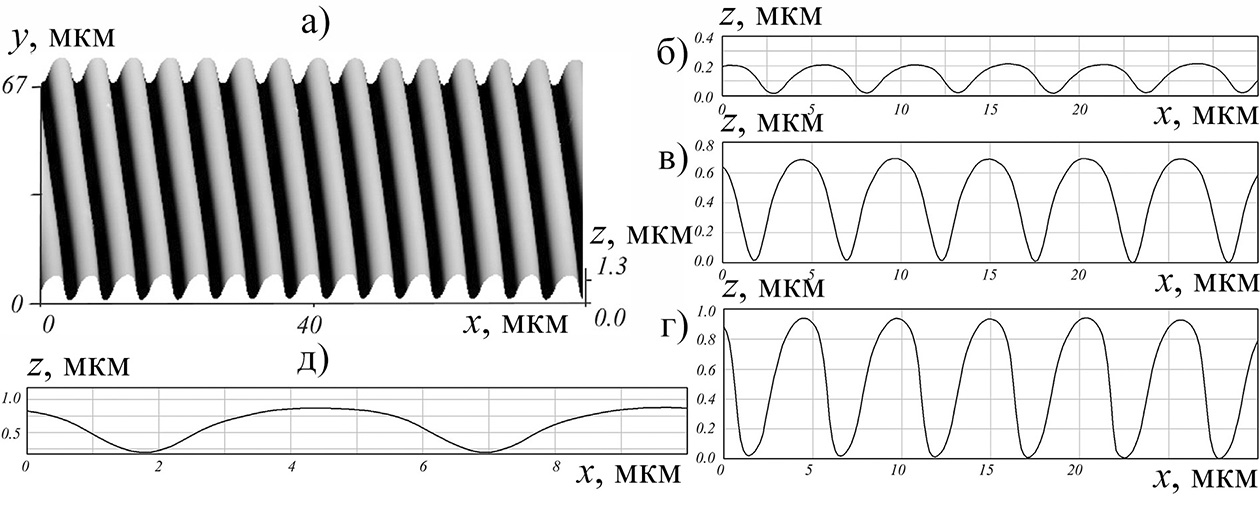
\includegraphics{1_chapter/DEBER_many_profiles_14pt_200}
	\vspace{0.2em}
	\caption{Профили периодических структур, полученных методом СЭЛТР в слое ПММА толщиной 900 нм при экспонировании вдоль серии параллельных линий при температуре 160~$^\circ$C: а) трехмерное изображение; б), в), г) профили, полученные при дозах экспонирования 0.05, 0.2 и 0.87 мкКл/см$\pp$ соответственно; д) изображение профиля в) в масштабе 1:1~\cite{Bruk_2016_mee}.}
	\label{fig:DEBER_many_profiles}
\end{figure}

\underline{\textbf{Вторая глава}} посвящена описанию существующих моделей и методов моделирования процессов, протекающих при СЭЛТР.
Основными процессами, влияющими на профиль линии в методе СЭЛТР, являются рассеяние электронного пучка в резисте и подложке, электронно-стимулированные разрывы молекул резиста, электронно-стимулированная термическая деполимеризация резиста, диффузия мономера и растекание резиста.
Некоторые из этих процессов достаточно хорошо изучены -- так, в настоящее время существуют высокоточные модели упругого и неупругого рассеяния электронного пучка в веществе.
В то же время, некоторые процессы являются изученными относительно слабо -- например, для описания электронно-стимулированных разрывов молекул резиста существует только макроскопический подход, основанный на анализе распределения энергии, выделившейся в слое резисте~\cite{Greeneich1979_Mf_Mn}.
Кинетические модели термической деполимеризации полимеров, в свою очередь, требуют задания различных констант, значения которых приведены в литературе лишь для некоторых частных случаев~\cite{Boyd_3, Mita_PMMA_zip_lengths_T}.
В отдельную группу можно выделить процессы диффузии мономера и растекания резиста -- для них существуют простые и в то же время достаточно точные модели~\cite{Fragala_3_diffusion, Leveder_2010, Kirchner_reflow}, однако, эти модели не могут быть использованы в исходном виде в силу неоднородности резиста в методе СЭЛТР.
Таким образом, для описания процессов, протекающих при сухом электронно-лучевом травлении резиста, требуется существенная доработка существующих моделей либо разработка на их основе новых моделей.

В \underline{\textbf{третьей главе}} описываются методы, которые использовались при разработке и верификации модели сухого электронно-лучевого травления резиста.
В соответствии с проведенными ранее экспериментами в данной работе в качестве резиста был выбран полиметилметакрилат (ПММА), в качестве материала подложки -- кремний~(Si).

Для моделирования рассеяния электронного пучка в системе ПММА/Si был реализован алгоритм на основе метода Монте-Карло. Для описания упругих процессов использовались моттовские сечения упругого рассеяния, сечения неупругого электрон-электронного рассеяния рассчитывались из функций потерь энергии ПММА и кремния.
Для повышения точности моделирования также учитывались неупругие процессы электрон-фононного и электрон-поляронного рассеяния в слое ПММА~\cite{Ciappa_2010}.

Для моделирования электронно-стимулированных разрывов молекул ПММА при повышенной температуре была разработана оригинальная микроскопическая модель.
В качестве приводящих к разрыву полимерных молекул в ней рассматривались процессы электрон-электронного рассеяния, и для моделирования электронно-стимулированных разрывов молекул ПММА была введена вероятность разрыва при электрон-электронном рассеянии $\ps$.
При заданной вероятности разрыва $\ps$ акты электрон-электронного рассеяния, приводящие к разрыву молекул, моделировались методом Монте-Карло:
\begin{equation} \label{eq:MC_9}
	\begin{aligned}
		\xi < \ps & \Rightarrow \text{разрыв молекулы} \\
		\xi \geq \ps & \Rightarrow \text{нет разрыва},
	\end{aligned}
\end{equation}
где $\xi$ -- случайное число из промежутка [0, 1).
Значения $\ps$ для различных температур были найдены путем моделирования эксперимента по вычислению радиационно-химического выхода разрывов молекул ПММА $\Gs$.
Значение $\Gs$, определяемое как число разрывов молекул, происходящих при выделении в слое полимерного резиста энергии 100~эВ, вычисляется экспериментально на основе значений среднечисловой молекулярной массы резиста до и после экспонирования~\cite{Greeneich1979_Mf_Mn}.
Для моделирования экспериментального значения $\Gs$ сначала на основе модели идеальной цепи проводилось моделирование слоя ПММА.
Далее моделировались акты электрон-электронного рассеяния, которые впоследствии сопоставлялись конкретным мономерам в модели слоя ПММА.
Это позволило при каждом значении $\ps$ промоделировать распределение молекулярной массы ПММА после экспонирования и затем промоделировать экспериментальное значение $\Gs$.
Так, для каждой температуры было подобрано значение $\ps$, обеспечивающее соответствие между промоделированным и экспериментальным~\cite{Charlesby_1964_Gs} значениями $\Gs$.
Было установлено, что экспериментально зарегистрированное увеличение $\Gs$ ростом температуры от 0 до 200~$^\circ$C может быть описано за счет увеличения вероятности разрыва молекулы ПММА при электрон-электронном рассеянии от 0.045 до 0.105.

Для моделирования электронно-стимулированной термической деполимеризации ПММА в процессе СЭЛТР использовалась кинетическая модель термической деполимеризации при возникновении активных центров деполимеризации в произвольных точках внутри полимерной молекулы~\cite{Boyd_3}.
В случае постоянной концентрации радикализованных молекул эта модель приводит к системе уравнений вида
%\begin{equation} \label{eq:moment_equation}
%	\frac{d M_i}{d t}=k_s\left(\frac{2}{i+1}-1\right) M_{i+1}+\frac{d M_0}{d t}-k_s M_1 - \frac{i}{\gamma}\left(k_s M_i+\frac{d M_{i-1}}{d t}\right) \quad(i \geq 1),
%\end{equation}
\begin{equation} \label{eq:moment_equation}
	\frac{d M_i}{d t} = k_\mathrm{S} \left(\frac{2}{i+1} - 1\right) M_{i+1} + \frac{d M_0}{d t} - k_\mathrm{S} M_1 - \frac{i}{\gamma}\left(k_\mathrm{S} M_i + \frac{d M_{i-1}}{dt}\right) \quad(i \geq 1),
\end{equation}
%где $k_\mathrm{S}$ -- константа скорости инициирования кинетической цепи при деполимеризации (число активных центров деполимеризации, появляющихся за 1 с, приходящееся на один мономер), $1/\gamma$ -- средняя длина кинетической цепи (среднее число свободных мономеров, образующихся в резисте вследствие возникновения одного активного центра деполимеризации), $M_i$ -- момент функции распределения молекулярной массы резиста порядка $i$ ($P_n$ -- число стабильных полимерных молекул степени полимеризации $n$):
где $k_\mathrm{S}$ -- константа скорости инициирования кинетической цепи при деполимеризации (число активных центров деполимеризации, появляющихся за 1 с, приходящееся на один мономер), $1/\gamma$ -- средняя длина кинетической цепи (среднее число свободных мономеров, образующихся вследствие возникновения одного активного центра деполимеризации), $M_i$ -- момент $i$-го порядка молекулярно-массового распределения полимера ($P_n$ -- число молекул степени полимеризации $n$):
\begin{equation}
	M_i=\sum_{n=2}^{\infty} n^i P_n.
\end{equation}
Данная система решалась численно для каждой ячейки размерами 100$\times$100$\times$5 нм$\ppp$ внутри слоя ПММА в предположении, что молекулярно-массовое распределение \linebreak ПММА описывалось функцией распределения Шульца-Цимма.
При этом значение $k_\mathrm{s}$ в каждой ячейке вычислялось исходя из предположения, что число активных центров деполимеризации, появлявшихся за 1~с в данной ячейке, равнялось числу промоделированных разрывов полимерных молекул в ячейке.
Значения средней длины кинетической цепи при деполимеризации ПММА были взяты из работы~\cite{Mita_PMMA_zip_lengths_T}.
Такой подход позволил промоделировать распределения среднечисловой молекулярной массы \linebreak ПММА в различные моменты процесса СЭЛТР (рисунок~\ref{fig:Mn_hist}).
\begin{figure}[t]
	\begin{center}
		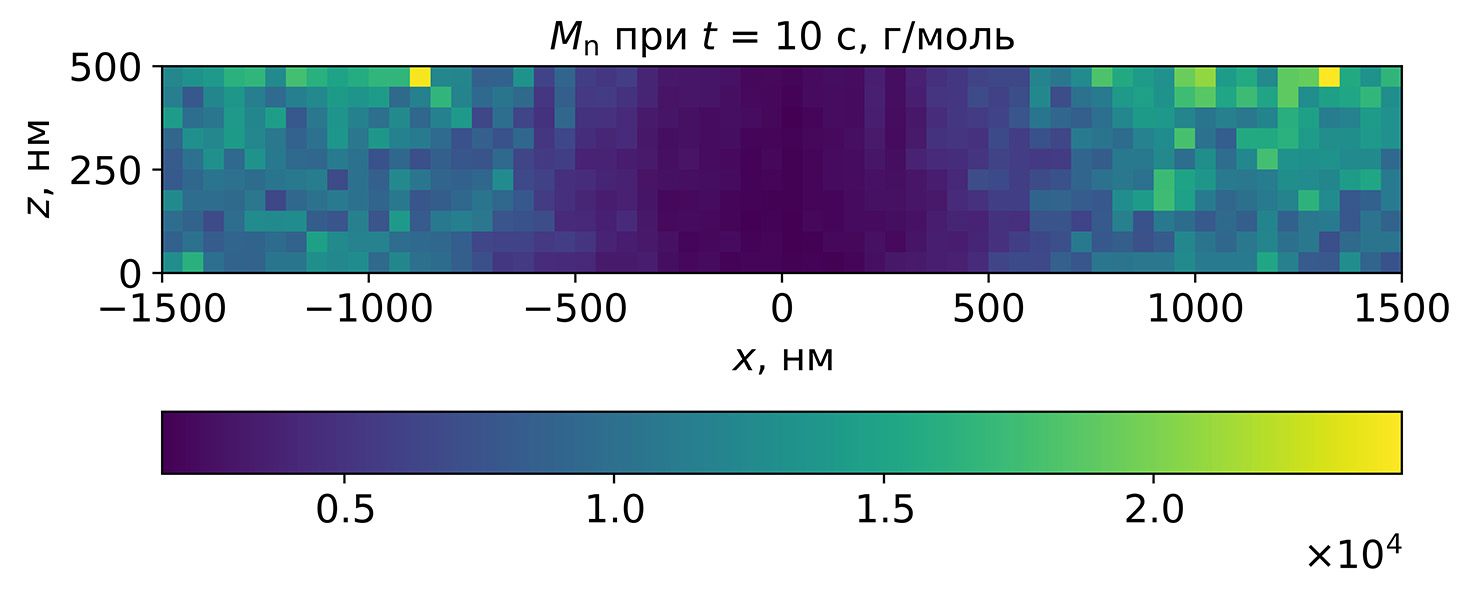
\includegraphics[width=0.7\linewidth]{MW/Mn_hist_10s_straight_200} \\
		\vspace{-3.7em} \text{\hspace{-26em} a)} \vspace{2.7em} \\
		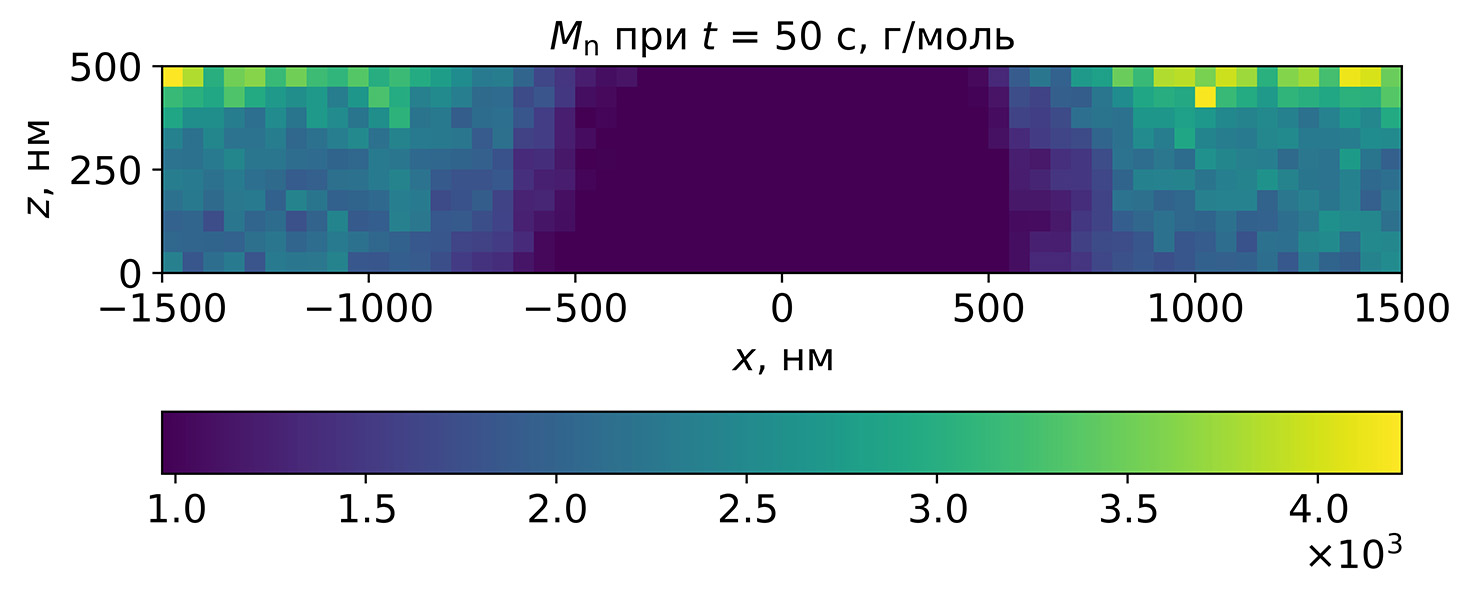
\includegraphics[width=0.7\linewidth]{MW/Mn_hist_50s_straight_200} \\
		\vspace{-3.7em} \text{\hspace{-26em} б)} \vspace{3.7em} \\
	\end{center}
	\vspace{-2.5em}
	\caption{Промоделированные распределения среднечисловой молекулярной массы ПММА при его экспонировании электронным лучом вдоль серии параллельных линий с расстоянием между линиями 3~мкм. Начальная среднечисловая молекулярная масса ПММА составляет примерно 271000, плотность тока экспонирования на единицу длины линии -- 30 пА/см, начальная энергия электронного пучка -- 20 кэВ, толщина слоя ПММА -- 500 нм, температура образца -- 130~$^\circ$C. Время экспонирования составляло 10~с (а) и 50~с (б). Моделирование проводилось в пределах одной линии с периодическими граничными условиями.}
	\label{fig:Mn_hist}
\end{figure}

Моделирование диффузии мономера, образующегося в слое ПММА в процессе деполимеризации, проводилось путем численного решения уравнения диффузии.
Для определения значений коэффициента диффузии мономера в слое ПММА использовались промоделированные распределения среднечисловой молекулярной массы \linebreak ПММА, а также значения и зависимости, приведенные в работах~\cite{Fragala_3_diffusion, Berens_diffusion_Mn}.
Моделирование показало, что за первые несколько секунд процесса СЭЛТР коэффициент диффузии снижается до значений, при которых время диффузии мономера, образующегося за 1~с экспонирования, из слоя ПММА толщиной в несколько сотен нанометров составляет менее 1~с.
Ввиду этого в дальнейшем считалось, что весь мономер, образующийся в процессе деполимеризации, мгновенно покидает слой ПММА, что приводит к образованию микрополостей.

%Распределения вязкости ПММА рассчитывались на основе промоделированных распределений среднечисловой молекулярной массы ПММА, а также значений и зависимостей, приведенных в работе~\cite{Leveder_2010}.
Для моделирования растекания слоя ПММА в процессе СЭЛТР был разработан подход на основе метода конечных элементов.
В данном подходе растекание слоя рассматривалось как процесс эволюции его поверхности под действием сил поверхностного натяжения.
При этом было необходимо учесть, что вследствие неоднородного распределения среднечисловой массы ПММА в процессе СЭЛТР вязкость ПММА также будет иметь неоднородное распределение~\cite{Leveder_2010}.
За счет этого различные участки поверхности слоя ПММА будут двигаться с различной скоростью под действием одной и той же силы.
Для учета этого эффекта вершинам поверхности слоя ПММА приписывались различные значения подвижности, определяющие связь между силой, действующей на вершину, и скоростью вершины.
Соотношение между локальным значением коэффициента вязкости ПММА и подвижностью вершин его поверхности было определено путем моделирования растекания прямоугольных решеток с однородным профилем вязкости аналитическим~\cite{Leveder_2010} и численным~\cite{Brakke_SE} методами.
Для значений коэффициента вязкости в диапазоне \linebreak 10$\pp$--10$^{\text{6}}$ Па$\cdot$с были подобраны значения подвижности вершин поверхности решеток, обеспечивающие соответствие между результатами моделирования, полученными обоими методами.
В результате было установлено, что подвижность вершин поверхности слоя ПММА $\mu$ может быть рассчитана из вязкости ПММА $\eta$ (в Па$\cdot$с) по формуле
\begin{equation}
	\mu \approx \frac{26.14}{\eta}.
\end{equation}
Полученное соотношение позволяло рассчитать значения подвижности для вершин поверхности сплошной структуры в слое ПММА с известным распределением вязкости и в дальнейшем численно промоделировать растекание этой структуры.

Однако, в методе СЭЛТР слой ПММА не является сплошным, и процессы растекания протекают за счет действия сил поверхностного натяжения как на поверхности слоя, так и на границах микрополостей внутри него.
Поэтому при моделировании процессов растекания использовалось приближение, состоящее в преобразовании слоя \linebreak ПММА в сплошную структуру.
Слой ПММА разделялся в плоскости $XY$ на участки размерами 100$\times$100 нм$\pp$, и для каждого участка на основе промоделированного распределения разрывов молекул ПММА и средней длины кинетической цепи при деполимеризации рассчитывались положения и объемы микрополостей (рисунок~\ref{fig:reflow_surface}а).
Далее точки поверхности слоя ПММА, соответствующие середине каждого участка по оси $X$, сдвигались вниз таким образом, чтобы объем призмы, образующейся под поверхностью слоя, был равен суммарному объему микрополостей на этом участке (рисунок~\ref{fig:reflow_surface}б).
Подвижности вершин полученной пилообразной структуры рассчитывались из распределения вязкости ПММА, после чего растекание структуры моделировалось численно в течение нужного промежутка времени.

\begin{figure}[h]
	\begin{minipage}{0.48\textwidth}
		\includegraphics[width=0.9\linewidth]{reflow/reflow_model_a_CIRCLES_4} \\
		\vspace{-28.5ex} \\ \text{\hspace{0em} a}) \\ \vspace{28.5ex}
	\end{minipage}
	\begin{minipage}{0.48\textwidth}
		\includegraphics[width=0.9\linewidth]{reflow/reflow_model_b} \\
		\vspace{-28.5ex} \\ \text{\hspace{-0.1em} б}) \\ \vspace{28.5ex}
	\end{minipage}
	\vspace{-3.5em}
	\caption{Иллюстрация подхода к моделированию растекания слоя ПММА со внутренними микрополостями.}
	\label{fig:reflow_surface}
\end{figure}

Объединение моделей рассеяния электронного пучка, электронно-стимулированных разрывов молекул ПММА, электронно-стимулированной термической деполимеризации ПММА, диффузии мономера и растекания слоя ПММА позволило создать модель модель сухого электронно-лучевого травления резиста.
На ее основе был разработан алгоритм моделирования профиля линии, получаемой методом СЭЛТР при произвольных параметрах процесса.
В данном алгоритме все время экспонирования разделялось на промежутки величиной 1~с, и на каждом промежутке последовательно выполнялись следующие действия:

\begin{enumerate}
	\item Моделирование рассеяния электронного пучка в системе ПММА/Si;
	\item Моделирование электронно-стимулированных разрывов молекул ПММА;
	\item Моделирование термической деполимеризации ПММА;
	\item Определение значений подвижности вершин поверхности слоя ПММА;
	\item Вычисление положений и объемов микрополостей в слое ПММА;
	\item Преобразование слоя ПММА в сплошную пилообразную структуру;
	\item Моделирование растекания пилообразной структуры;
	\item Определение нового положения поверхности слоя ПММА.
\end{enumerate}
По истечении времени экспонирования моделировалось растекание слоя ПММА при охлаждении образца.

\underline{\textbf{В четвертой главе}} приводятся результаты  диссертационной работы.
Описывается верификация разработанной модели сухого электронно-лучевого травления резиста, а также ее применение для определения предельного разрешения метода СЭЛТР.
Помимо этого, разработанная модель используется для исследования влияния флуктуаций параметров процесса СЭЛТР на конечный профиль получаемой линии, а также для определения параметров процесса СЭЛТР для формирования синусоидальных дифракционных и голографических элементов.

Для верификации разработанной модели методом СЭЛТР были получены периодические структуры в слое ПММА на кремниевой подложке.
Экспонирование производилось в рабочей камере растрового электронного микроскопа CAMSCAN S-4, который был модифицирован для возможности нагрева образца, начальная толщина слоя ПММА составляла 500 нм.
Давление в камере микроскопа поддерживалось на уровне 10$^\text{-5}$ мбар, энергия электронного пучка составляла 20 кэВ, диаметр пучка -- \linebreak около 600 нм.
Экспонирование резиста производилось ``в кадр'' (вдоль серии параллельных линий), размеры кадра составляли 2.4$\times$1.9~мм$\pp$, число линий в кадре равнялось 625.
Ток экспонирования $I$ находился в диапазоне 4.56--5.62 нА, время экспонирования $t_\mathrm{exp}$ варьировалось от 100 до 200 с, таким образом, доза экспонирования на единицу длины линии $D_\mathrm{l}$ составляла 3.00--7.38~нКл/см.
Температура подложки образцов при экспонировании $T$ варьировалась от 130 до 150~$^\circ$C, скорость охлаждения подложки после экспонирования составляла около 0.2~$^\circ$C/с.
Профили линий были получены методом атомно-силовой микроскопии с использованием микроскопа Nanopics~2100.

Для снижения требуемого машинного времени моделирование проводилось для участка одной линии длиной 100 нм, влияние соседних линий учитывалось за счет использования периодических граничных условий.
Число разрывов молекул ПММА, локальная среднечисловая молекулярная масса ПММА и объемы микрополостей вычислялись для ячеек размерами 100$\times$100$\times$5 нм$\ppp$ (по осям $X$, $Y$ и $Z$, соответственно).
Для учета стохастической природы алгоритма моделирования для каждого набора параметров экспонирования проводилось 100 независимых моделирований.
Далее на основе 100 полученных профилей рассчитывался усредненный промоделированный профиль (слово ``усредненный'' в дальнейшем будет опускаться).
Сравнение экспериментальных и промоделированных профилей приведено на рисунке~\ref{fig:DEBER_2_profiles}.
Высокая степень воспроизведения экспериментальных профилей указывает на достоверность разработанной модели процесса СЭЛТР.

\begin{figure}[h]
	\begin{minipage}{0.48\textwidth}
		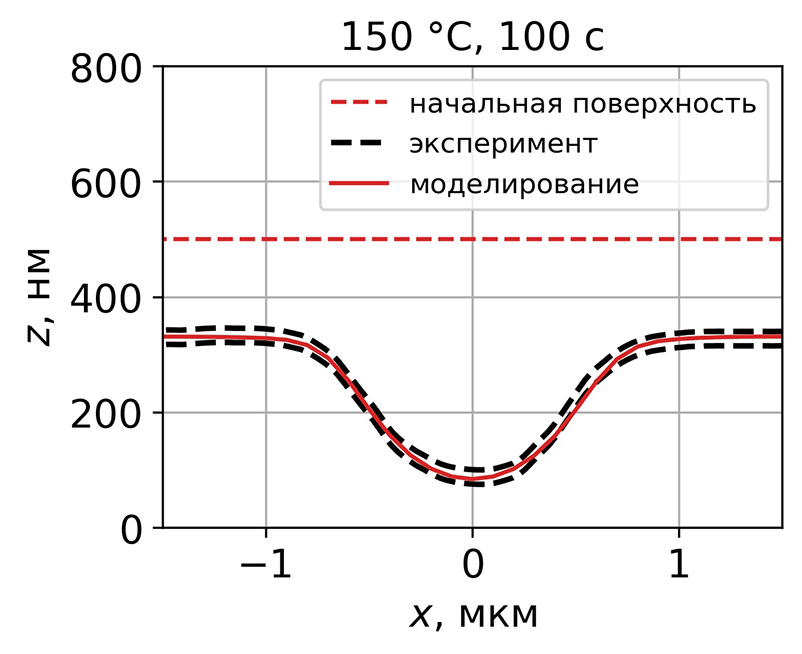
\includegraphics[width=0.9\linewidth]{DEBER_verification/150C_100s_14_FINAL_200} \\
		\vspace{-12em} \\ \text{\hspace{0em} a}) \\ \vspace{12em}
	\end{minipage}
	\begin{minipage}{0.48\textwidth}
		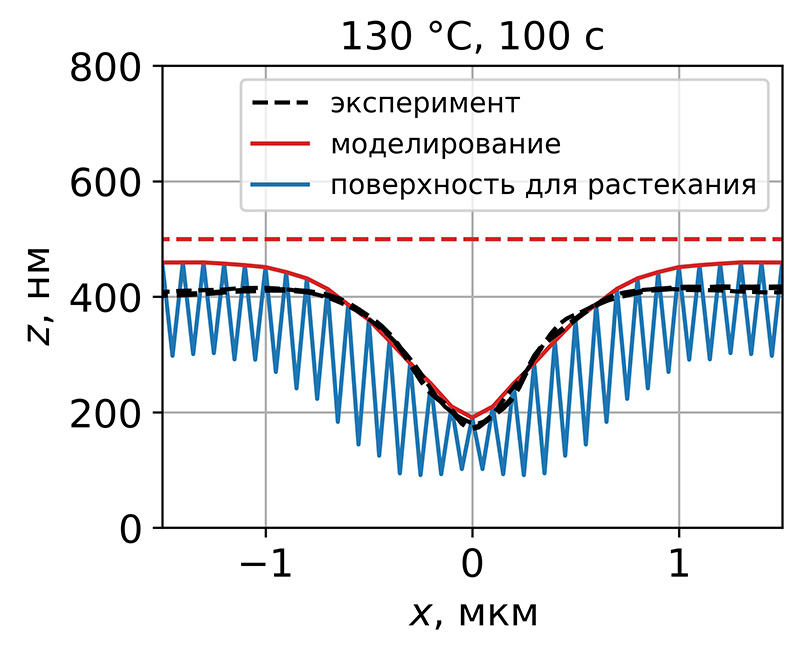
\includegraphics[width=0.9\linewidth]{DEBER_verification/130C_100s_14_FINAL_200} \\
		\vspace{-12em} \\ \text{\hspace{-0.1em} б}) \\ \vspace{12em}
	\end{minipage}
	\vspace{-3.5em}
	\caption{
		Верификация разработанной модели процесса СЭЛТР -- сравнение экспериментальных и промоделированных профилей для следующих условий экспонирования: a) $T$ = 150~$^\circ$C, $t_\mathrm{exp}$ = 100 c, $D_\mathrm{l}$ = 3.00 нКл/см; б) $T$ = 130~$^\circ$C, $t_\mathrm{exp}$ = 100 c, $D_\mathrm{l}$ = 3.12 нКл/см.
		В обоих случаях начальная энергия электронного пучка составляла 20 кэВ, диаметр пучка -- около 600~нм, скорость охлаждения подложки после экспонирования -- примерно 0.2~$^\circ$C/с.
		Черная пунктирная линия обозначает профили, полученные в эксперименте, красная пунктирная линия -- начальное положение поверхности ПММА, синяя линия -- пилообразную поверхность, использовавшуюся при моделировании растекания слоя ПММА со внутренними микрополостями.}
	\label{fig:DEBER_2_profiles}
%	\vspace{1em}
\end{figure}

На основе разработанной модели были выявлены два пути увеличения разрешения метода СЭЛТР.
Во-первых, латеральное разрешение метода может быть увеличено за счет использования узкого высокоэнергетического пучка.
Малый диаметр пучка позволит локализовать большинство разрывов молекул резиста в центре линии, что вызовет интенсивную деполимеризацию, образование микрополостей и снижение вязкости резиста в этой области.
Помимо этого, за счет высокой энергии пучка будет снижено число разрывов на краях линии, вызванных обратно отраженными электронами.
При этом будет необходимо подобрать время экспонирования так, чтобы на момент остывания образца микрополости в центре линии заполнились, а микрополости на краях -- остались незаполненными.
Во-вторых, использование узкого низкоэнергетического пучка также может увеличить латеральное разрешение метода СЭЛТР.
При низкой энергии первичных электронов все разрывы полимерных молекул будут происходить вблизи центра линии за счет относительно небольшой глубины проникновения электронов.
В этом случае микрополости будут формироваться только в ограниченной области вблизи центра линии, что исключит проседание краев линии.
На рисунке~\ref{fig:DEBER_resolution} приведены результаты моделирования профилей, полученных методом СЭЛТР с латеральным разрешением, увеличенным обоими вышеописанными способами.
На основе результатов моделирования было установлено, что минимальная ширина на полувысоте и максимальный угол наклона стенок канавки, получаемой методом СЭЛТР при экспонировании в линию, составляют около 300 нм и 70$^\circ$ соответственно.

\begin{figure}[h]
	\begin{minipage}{0.48\textwidth}
		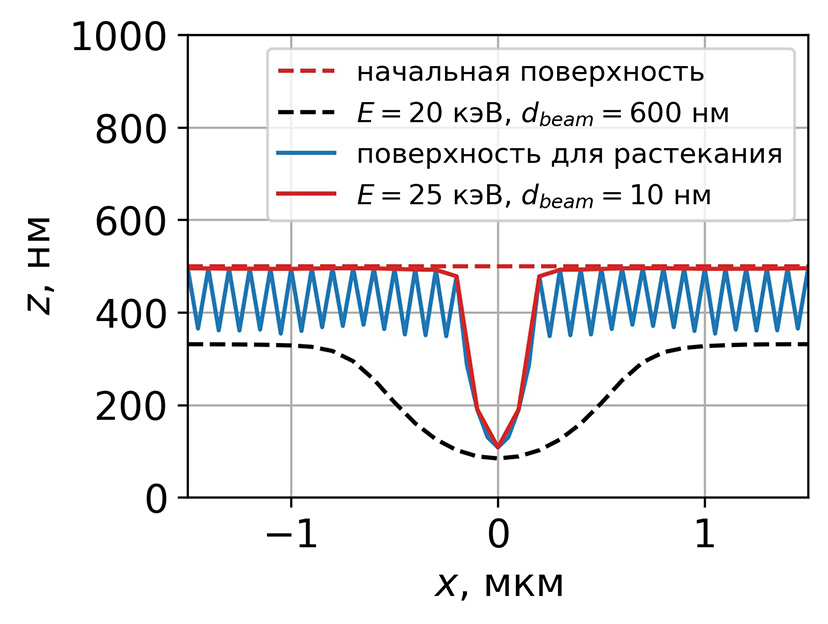
\includegraphics[width=\linewidth]{DEBER_resolution/resolution_25_um_200} \\
		\vspace{-28.7ex} \\ \text{\hspace{0em} a}) \\ \vspace{28.7ex}
	\end{minipage}
	\begin{minipage}{0.48\textwidth}
		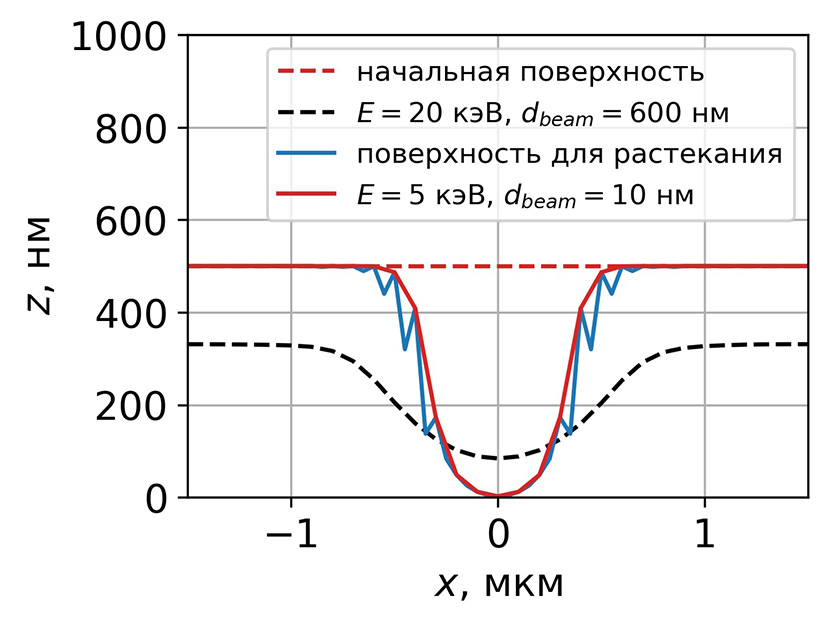
\includegraphics[width=\linewidth]{DEBER_resolution/resolution_5_um_200} \\
		\vspace{-28.7ex} \\ \text{\hspace{-0.1em} б}) \\ \vspace{28.7ex}
	\end{minipage}
	\vspace{-3.5em}
	\caption{
		Моделирование профилей, полученных методом СЭЛТР при использовании узкого пучка с энергией 25 кэВ (а) и 5 кэВ (б).
		Диаметр пучка составлял 10 нм, температура образцов -- 150~$^\circ$C/с, начальная толщина слоя ПММА -- 500 нм.
		Экспонирование производилось вдоль одиночной линии, плотность тока экспонирования на единицу длины линии составляла 30~пА/см, скорость охлаждения образцов -- 10~$^\circ$C/с.}
	\label{fig:DEBER_resolution}
\end{figure}

Разработанный алгоритм моделирования профиля линии, получаемой методом СЭЛТР, также был использован для исследования влияния флуктуаций параметров экспонирования на профиль линии.
Это позволило сформулировать требования к стабильности параметров экспонирования в методе СЭЛТР: для получения необходимого профиля флуктуации энергии пучка, тока экспонирования и температуры образца должны составлять не более 0.5~кэВ, 0.1~нА и 1~$^\circ$C соответственно.
Такие флуктуации параметров экспонирования приводят к флуктуациям высоты точек промоделированного профиля, сопоставимым со среднеквадратичным отклонением высоты точек при моделировании (около 2 нм).
Максимально допустимая флуктуация скорости охлаждения образца, определенная аналогичным образом, составляет 0.1~$^\circ$C/с.

Проведенные эксперименты показали, что при экспонировании резиста в методе СЭЛТР ``в кадр'' профиль получаемого рельефа имеет волнообразную форму.
Вследствие этого целесообразным являлось изучение возможности использования метода СЭЛТР для формирования синусоидальных голографических решеток, широко применяющихся в оптике.
На основании результатов моделирования можно заключить, что методом СЭЛТР в слое ПММА могут быть получены синусоидальные решетки с плотностью штрихов до 2000 1/мм.
Как показано на рисунке~\ref{fig:DEBER_holo_2um}, синусоидальный профиль рельефа может быть получен как при наличии микрополостей в слое ПММА на момент остывания образца (рисунки~\ref{fig:DEBER_holo_2um}a, \ref{fig:DEBER_holo_2um}б), так и при их отсутствии (рисунки~\ref{fig:DEBER_holo_2um}в, \ref{fig:DEBER_holo_2um}г).
При этом среднеквадратичное отклонение точек промоделированных профилей от графика функции синус составляет менее 5\% от глубины решетки.
Полученные в ПММА синусоидальные решетки могут быть в дальнейшем покрыты металлом или перенесены в металл путем травления в реакторе индуктивно-связанной плазмы~\cite{Bruk_2016_mee}, что может быть использовано для формирования отражательных синусоидальных голографических решеток.

\begin{figure}[h!]
	\begin{minipage}{0.48\textwidth}
		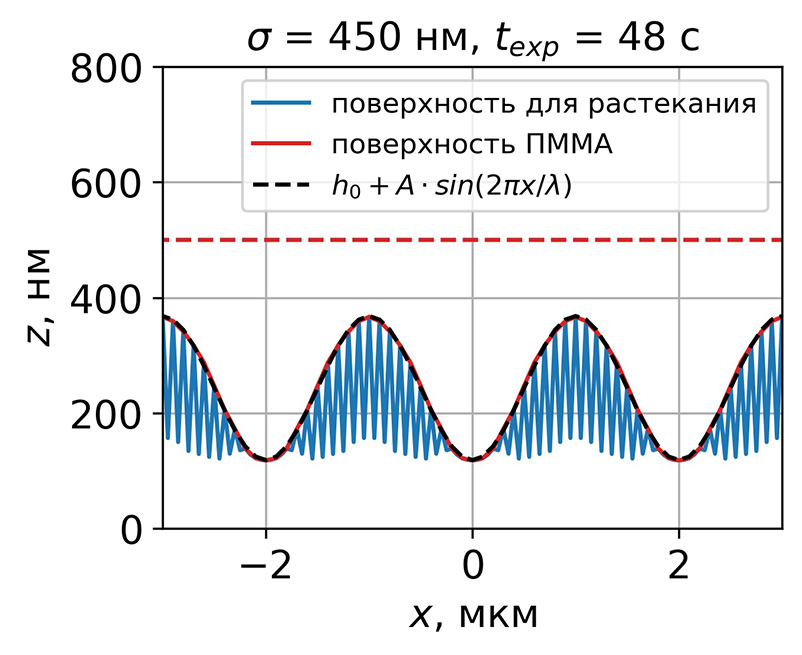
\includegraphics[width=0.9\linewidth]{DEBER_holo/2_um/holo_1C_s450_48s_um_200} \\
		\vspace{-12em} \\ \text{\hspace{0em} a}) \\ \vspace{12em}
	\end{minipage}
	\begin{minipage}{0.48\textwidth}
		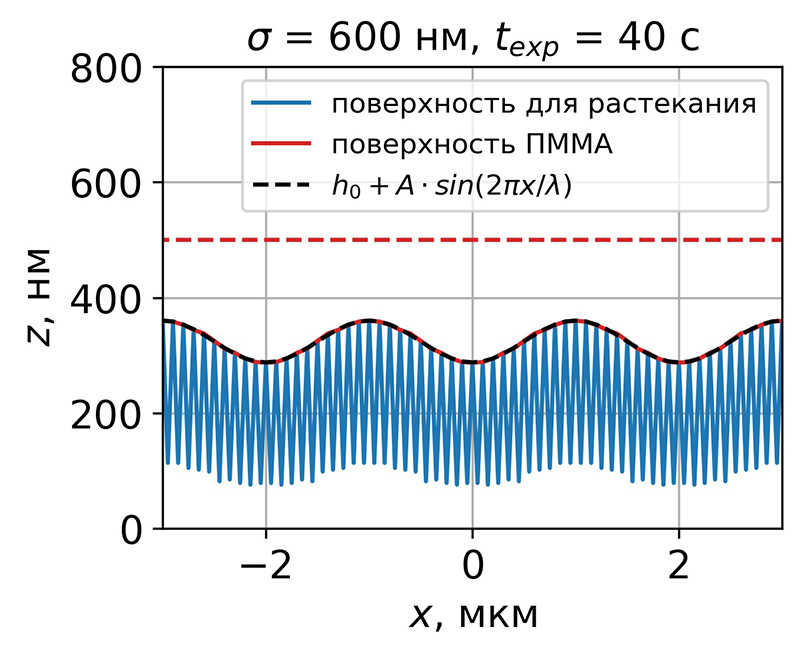
\includegraphics[width=0.9\linewidth]{DEBER_holo/2_um/holo_1C_s600_40s_um_200} \\
		\vspace{-12em} \\ \text{\hspace{-0.1em} б}) \\ \vspace{12em}
	\end{minipage}
	
	\vspace{-3.5em}
	
	\begin{minipage}{0.48\textwidth}
		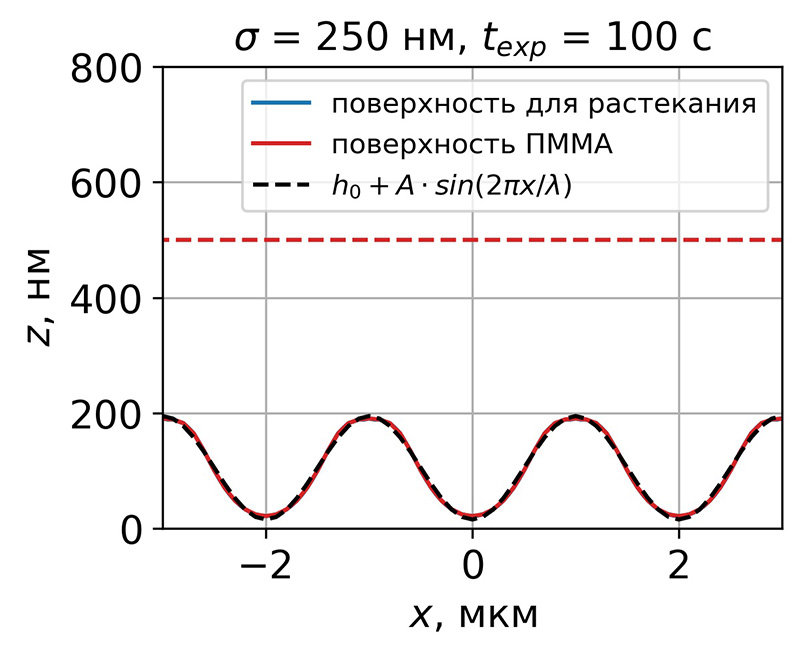
\includegraphics[width=0.9\linewidth]{DEBER_holo/2_um/holo_10C_s250_100s_um_200} \\
		\vspace{-12em} \\ \text{\hspace{0em} в}) \\ \vspace{12em}
	\end{minipage}
	\begin{minipage}{0.48\textwidth}
		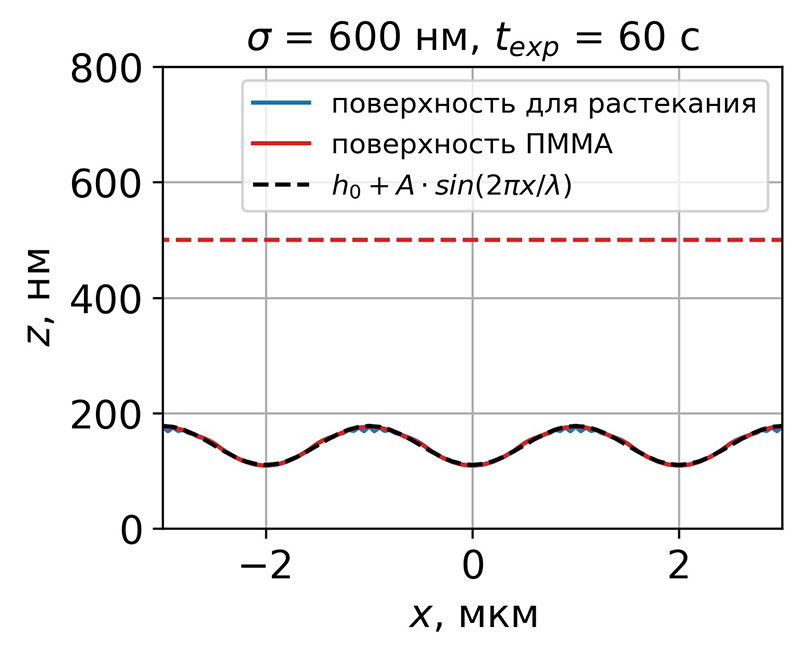
\includegraphics[width=0.9\linewidth]{DEBER_holo/2_um/holo_1C_s600_60s_um_200} \\
		\vspace{-12em} \\ \text{\hspace{-0.1em} г}) \\ \vspace{12em}
	\end{minipage}
	\vspace{-3.5em}
	\caption{Промоделированные синусоидальные профили с пространственным периодом $\lambda$ = 2~мкм, полученные методом СЭЛТР в слое ПММА с начальной толщиной 500 нм. Температура образцов при экспонировании составляла 150~$^\circ$C, плотность тока экспонирования на единицу длины линии -- 30 пА/см, начальная энергия электронного пучка -- 20 кэВ, распределение плотности тока в пучке считалось нормальным со среднеквадратичным отклонением $\sigma$. Значения $\sigma$ и $t_\mathrm{exp}$ были подобраны для получения синусоидального профиля. После экспонирования образец а) охлаждался со скоростью 10~$^\circ$C/с, образцы б)-г) -- со скоростью 1~$^\circ$C/с. Черная пунктирная линия обозначает аппроксимацию промоделированного профиля функцией синус.}
	\label{fig:DEBER_holo_2um}
\end{figure}

Приведенные выше промоделированные профили относятся к структурам, получаемым методом СЭЛТР при экспонировании вдоль серии параллельных линий либо вдоль одиночной линии.
Однако, при моделировании может быть заложено произвольное распределение плотности тока по области экспонирования (рисунок~\ref{fig:DEBER_multibeam}).
За счет этого разработанные в данной работе модель СЭЛТР и алгоритм моделирования профиля линии, получаемой в этом процессе, могут использоваться при определении параметров для формирования методом СЭЛТР необходимого профиля.
В самом деле, для получения методом СЭЛТР рельефа, профиль которого согласуется с предельным разрешением метода, параметры экспонирования и последующего охлаждения образца могут быть подобраны путем многократного моделирования конечного профиля с учетом выявленных особенностей метода.

\begin{figure}[h]	
	\begin{minipage}{0.48\textwidth}
		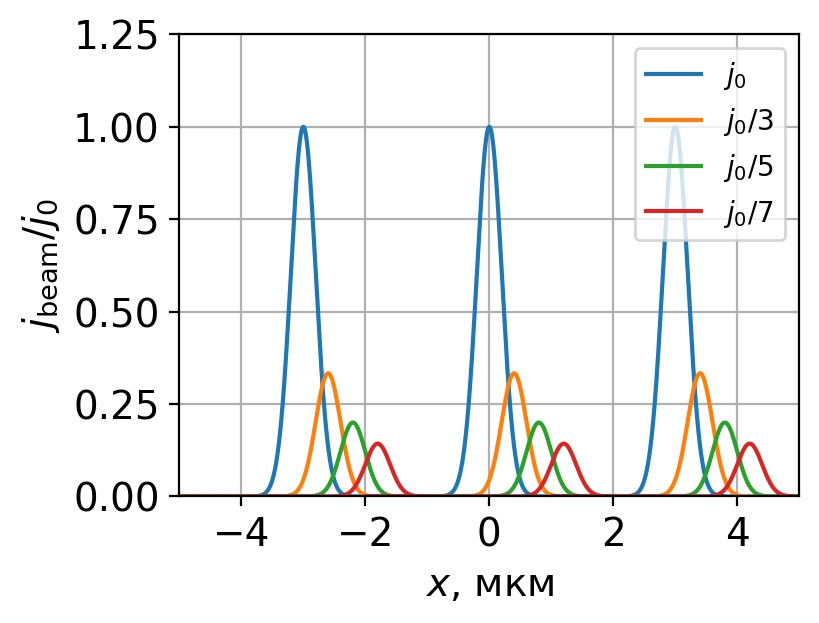
\includegraphics[width=0.9\linewidth]{DEBER_asymmetric/asymmetric_beam_200} \\
		\vspace{-12em} \\ \text{\hspace{0em} а}) \\ \vspace{12em}
	\end{minipage}
	\begin{minipage}{0.48\textwidth}
		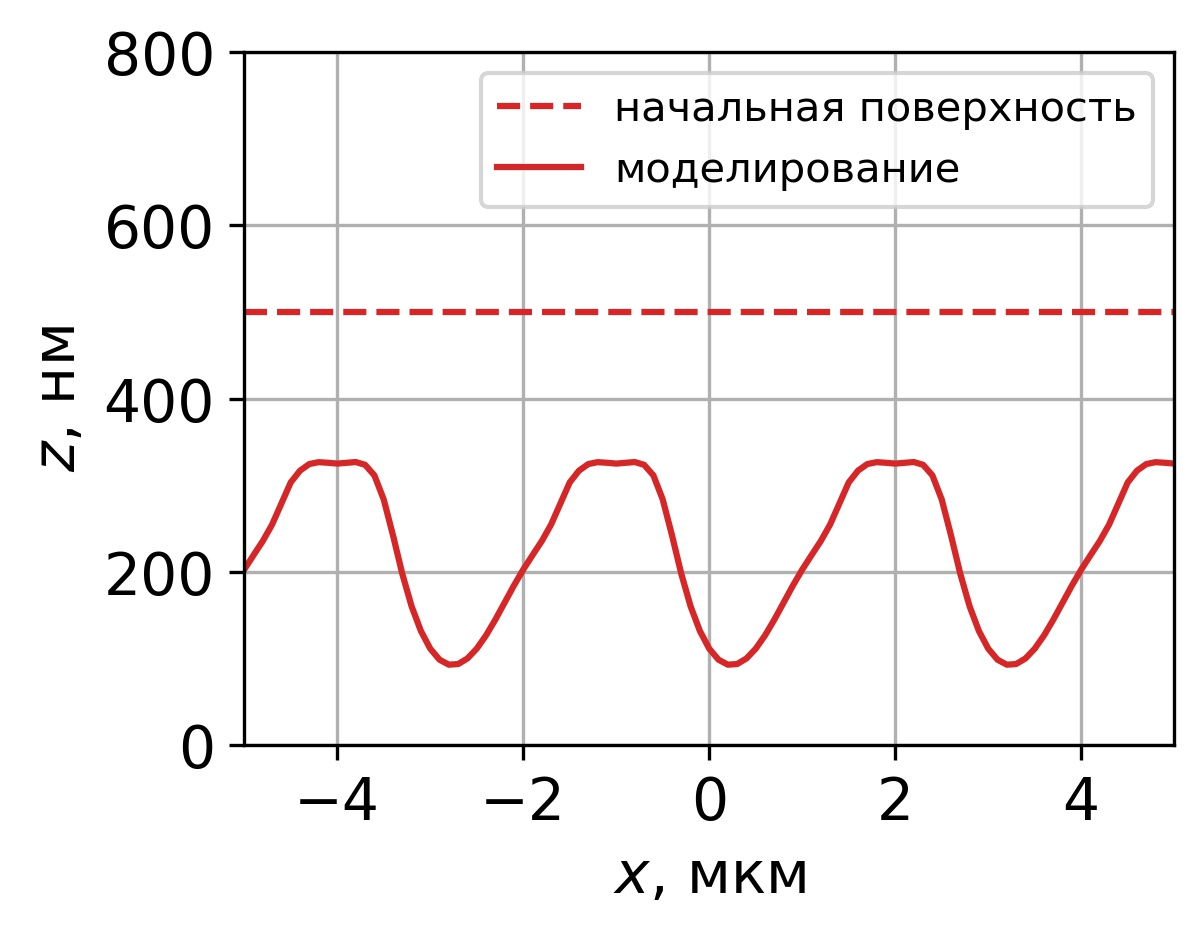
\includegraphics[width=0.9\linewidth]{DEBER_asymmetric/asymmetric_profile_200} \\
		\vspace{-12em} \\ \text{\hspace{-0.1em} б}) \\ \vspace{12em}
	\end{minipage}
	\vspace{-3.5em}
	\caption{Демонстрация возможностей разработанного алгоритма -- моделирование профилей (б), полученных в слое ПММА с начальной толщиной 500~нм методом СЭЛТР при экспонировании по области с плотностью тока в пучке, описывающейся суммой нескольких функций Гаусса (a). Температура образца при экспонировании -- 150~$^\circ$C/с, время экспонирования -- 100 с, плотность тока экспонирования на единицу длины линии -- 30 пА/см.}
	\label{fig:DEBER_multibeam}
	\vspace{2em}
\end{figure}

%% Согласно ГОСТ Р 7.0.11-2011:
%% 5.3.3 В заключении диссертации излагают итоги выполненного исследования, рекомендации, перспективы дальнейшей разработки темы.
%% 9.2.3 В заключении автореферата диссертации излагают итоги данного исследования, рекомендации и перспективы дальнейшей разработки темы.
\chapter*{Заключение}						% Заголовок
\addcontentsline{toc}{chapter}{Заключение}	% Добавляем его в оглавление
В настоящей диссертации рассмотрена возможность использования узкозонных полупроводников для межзонной лазерной генерации в ТГц диапазоне. Особое внимание уделено процессам оже-рекомбинации и рекомбинации с испусканием плазмонов, поскольку именно они будут определять пороговые токи ТГц лазерных диодов. Так как подавление оже-рекомбинации ожидается в материалах с дираковским законом дисперсии $E = \pm\sqrt{v_0^2 p^2 + E_g^2/4}$, были рассмотрены случаи дираковского и приближённо дираковского закона дисперсии на примере графена и квантовых ям \HgCdTe{}.

В случае дираковского закона дисперсии трёхчастичная оже-рекомбинация запрещена законами сохранения (кроме коллинеарных процессов в бесщелевом случае), и темп оже-рекомбинации определяется многочастичными процессами. Для учёта этих процессов нами разработан подход, основанный на методе неравновесных функций Грина и самосогласованном $GW$-приближении. С использованием этого подхода рассчитаны времена оже-рекомбинации в нелегированном графене со слабой инверсией населённостей и продемонстрировано их согласие с экспериментальными данными. Полученные времена составляют около 1--3 пс при комнатной температуре в зависимости от диэлектрической проницаемости окружающего материала. Это свидетельствует о том, что для бесщелевого дираковского спектра запрет на оже-рекомбинацию со стороны законов сохранения фактически исчезает из-за эффектов уширения спектра, связанных с рассеянием носителей друг на друге. Также мы сравнили разработанный нами метод расчёта темпа оже-рекомбинации с более простыми методами, использовавшимися в литературе, и показали, что более простые методы могут давать ошибку в несколько раз из-за неучтённых или некорректно учтённых многочастичных эффектов, таких как уширение и искривление спектра носителей, а также динамическое экранирование кулоновского взаимодействия. 

Наличие запрещённой зоны в дираковском спектре приводит к подавлению оже-рекомбинации даже в случае, когда трёхчастичные оже-процессы разрешены из-за отклонений реального закона дисперсии от дираковского, как показано нами на примере квантовых ям \HgCdTe{}. Рассчитанные пороговые энергии оже-рекомбинации в ямах нормальной зонной структуры достигают половины запрещённой зоны и более, что обусловлено близкими эффективными массами электронов и дырок (в отличие от трёхмерных полупроводников \AIIIBV{}) и непараболичностью закона дисперсии. Для ям с шириной запрещённой зоны в диапазоне 6--10 ТГц такие пороговые энергии соответствуют подавлению оже-рекомбинации на полтора-два порядка при 77 К по сравнению со случаем большой электрон-дырочной асимметрии, реализующимся в ямах инвертированной зонной структуры. Это подтверждается рассчитанными временами оже-рекомбинации, достигающими сотен пс при 77 К в ямах ТГц диапазона с нормальной зонной структурой, при том что в ямах с инвертированной зонной структурой эти времена составляют около 1 пс.

Помимо оже-рекомбинации, также была исследована рекомбинация с испусканием двумерных плазмонов. На примере квантовых ям \HgCdTe{} продемонстрировано, что существует некоторая пороговая концентрация носителей, ниже которой межзонные переходы с испусканием плазмонов в первом приближении невозможны (т. е. если не учитывать неопределённость энергии плазмонов из-за конечного времени жизни). Эта пороговая концентрация определяется условием пересечения закона дисперсии плазмонов с областью межзонных переходов в пространстве $(\vec{q}, \omega)$. При концентрации носителей выше пороговой плазмонная рекомбинация в квантовых ямах \HgCdTe{} оказывается быстрее оже-рекомбинации и имеет характерные времена порядка сотен фемтосекунд при 77 К; при концентрациях ниже пороговой плазмонная рекомбинация замедляется до 1 нс и более при 77 К и оказывается медленнее оже-рекомбинации. По нашим расчётам, при обеспечении достаточно низких оптических потерь за пределами активной среды пороговые концентрации для достижения лазерной генерации при 77 К в ямах \HgCdTe{} нормальной зонной структуры оказываются ниже пороговых концентраций для плазмонной рекомбинации, за исключением наиболее узкозонных ям.

Пороговая концентрация для плазмонной рекомбинации сильно чувствительна к поведению зонной структуры в области больших квазиимпульсов. Так, наличие побочного локального максимума в валентной зоне квантовых ям \HgCdTe{} снижает пороговые концентрации для плазмонной рекомбинации примерно на порядок по сравнению с дираковским законом дисперсии. Однако такая рекомбинация с участием дырок из побочного максимума валентной зоны имеет энергетический порог, равный разности энергий между основным и побочным максимумами, поэтому плазмонная рекомбинация может быть подавлена при низких температурах даже при превышении пороговой концентрации.

Рассчитанные времена рекомбинации в графене и квантовых ямах \HgCdTe{} были использованы для оценки пороговых токов ТГц лазерных диодов на основе этих материалов. Полученные значения при 77 К составляют сотни А/см$^2$ на одну квантовую яму и единицы кА/см$^2$ на один графеновый слой. Это свидетельствует в пользу достижимости межзонной ТГц генерации при азотной температуре, хотя окончательный ответ на этот вопрос требует аккуратного моделирования конкретной конструкции лазера. При 300 К достижению ТГц усиления в квантовых ямах \HgCdTe{} препятствует межподзонное и друдевское поглощение, а в графене пороговые токи составляют около 50 кА/см$^2$ на один графеновый слой, поэтому межзонная ТГц генерация в непрерывном режиме, скорее всего, возможна лишь при криогенных температурах. Достижимые частоты генерации в квантовых ямах \HgCdTe{} ограничены снизу областью сильного решёточного поглощения и составляют около 6 ТГц. В гексагональном нитриде бора, использующемся в качестве диэлектрика в высококачественных графеновых гетероструктурах, область сильного решёточного поглощения лежит выше ТГц диапазона, поэтому для графена минимальная частота генерации будет ограничена друдевским поглощением в волноводных слоях и самом графене и может быть меньше 6 ТГц при достаточно низких температурах.

На основании полученных результатов можно сформулировать общие рекомендации по проектированию ТГц лазерных диодов. Для достижения ТГц лазерной генерации на межзонных переходах в узкозонных материалах и минимизации пороговых токов требуется обеспечить подавление основных механизмов безызлучательной рекомбинации: оже-рекомбинации и рекомбинации с испусканием плазмонов. Этому благоприятствуют следующие факторы:
\begin{itemize}
\item наличие ненулевой запрещённой зоны;
\item дираковский закон дисперсии в как можно более широком диапазоне энергий;
\item отсутствие в этом диапазоне энергий каких-либо других зон/подзон, кроме нижней подзоны зоны проводимости и верхней подзоны валентной зоны;
\item низкие оптические потери в резонаторе и, соответственно, низкие пороговые концентрации носителей для достижения лазерной генерации;
\item низкий уровень остаточного легирования активной среды;
\item криогенные температуры.
 \end{itemize}

В заключение обсудим возможности дальнейшего развития темы исследования. С теоретической точки зрения представляет интерес обобщение разработанного метода расчёта темпа оже-рекомбинации с учётом многочастичных эффектов на случай сильного межэлектронного взаимодействия. Для этого требуется использование ещё более продвинутых приближений, нежели самосогласованное $GW$-приближение, и возникает проблема сохранения разумной вычислительной сложности. Также разработанный метод можно применить для определения точной границы между режимом, когда основной вклад в темп оже-рекомбинации связан с многочастичными эффектами, и режимом, когда основной вклад в темп оже-рекомбинации определяется отклонением закона дисперсии от дираковского. Другой важной теоретической проблемой для узкозонных материалов является корректный учёт динамического экранирования в условиях сильной инверсии населённостей, при которой возможно появление незатухающих плазмонов и зануление диэлектрической проницаемости на действительных частотах.

С практической точки зрения интересно применение результатов настоящей диссертации для моделирования конкретных конструкций ТГц лазеров на основе узкозонных материалов, поиск оптимального состава активной среды, а также исследование возможности ТГц генерации на плазмонных модах в двумерных материалах.
\urlstyle{rm}                               % ссылки URL обычным шрифтом
\insertbiblioother
\newrefcontext[labelprefix=A]
\printbibliography[keyword=biblioauthor,title=\authorbibtitle,resetnumbers]
\AtNextBibliography{\defcounter{maxnames}{666}}
%\printbibliography[keyword=biblioauthor,title=\authorbibtitle,resetnumbers]
%\insertbiblioauthor
\end{document}